\documentclass[serif]{beamer}

\usepackage[UTF8,noindent]{ctexcap}
\usepackage{amsmath}
%\usepackage{mathabx}
%\usepackage{tikz}
%\usetikzlibrary{mindmap,trees}
\usetheme{cambridgeUS}
%\usepackage{verbatim}

\title{中学数学课堂教学中提高记忆效能策略的研究}
\author{徐希来}
\institute{数学科学学院\\华东师范大学}
\date{\scriptsize {\today}}
\titlegraphic{
\includegraphics[width=0.32\textwidth]{ECNUred.jpg}}
\subject{数学与记忆}
\keywords{记忆,工作记忆,元记忆,数学记忆策略}
\logo{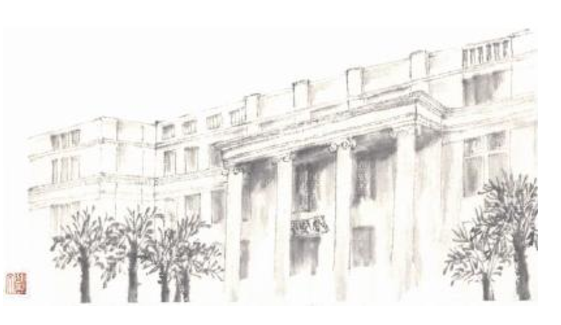
\includegraphics[scale=0.5]{WSbuilding.pdf}}

\begin{document}

  %\frame{\titlepage}  等效于\maketitle
  \begin{frame}
     \titlepage
  \end{frame}

  \begin{frame}\frametitle{目录}
  	\tableofcontents[hideallsubsections]%[part=1,pausesections]
  \end{frame}
  
  \section{研究的背景与意义}
  \subsection{研究的背景}
  
  \begin{frame}{研究背景与目的}
      \begin{itemize}
  \small{\item 记忆表现很大程度上影响着你的思维品质、学习能力
      	     \item 记忆以其特有的方式影响着数学学习
      	     \item 记忆不像肌肉那样可以通过重复锻炼而得到改善,除非在此过程中发明了一些可用于其他领域的记忆策略或方法
      	     \item 记忆策略的偏好影响你处理语义符号信息和视觉图像信息的能力
      	     }
      \end{itemize}
      \pause
      \begin{block}{研究目的}
      	通过优化记忆策略提高数学学习中的\\
      	记忆效率\tiny{(怎样更轻松快捷的记忆)}\\
      	\normalsize{记忆效果}\tiny {(怎样使记忆更具持效性、更易于提取)}
      \end{block}
  \end{frame}
  
  \begin{frame}{记忆与数学}
       \begin{figure}[t]
       	     \centering
       	    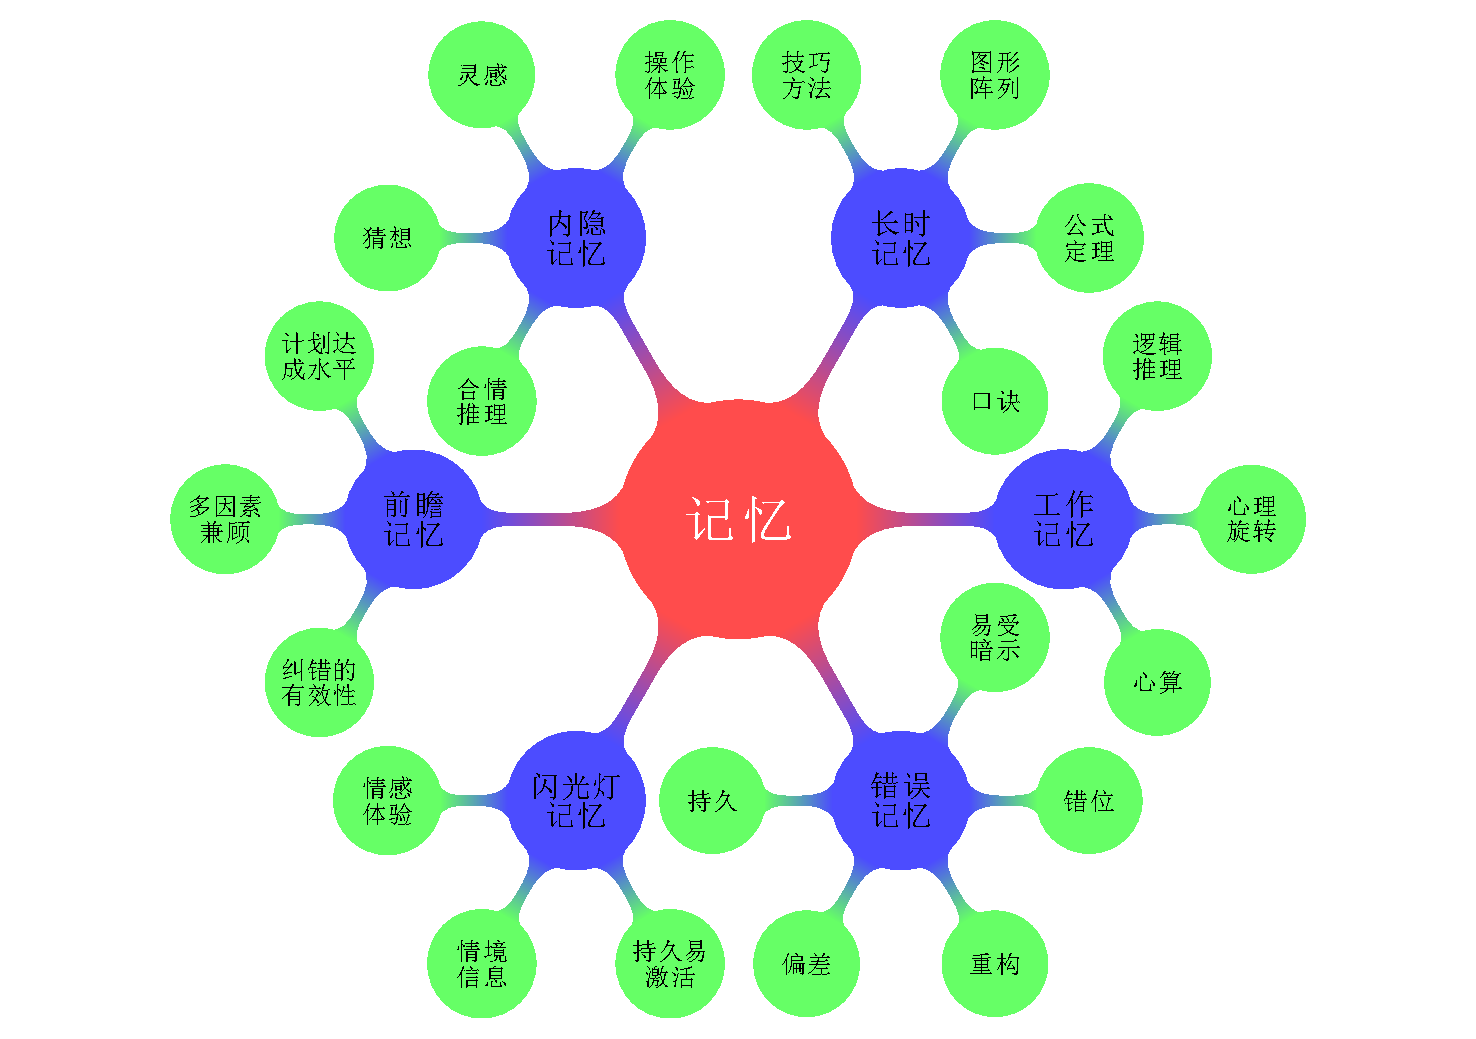
\includegraphics[scale=0.4]{memory.pdf}
       \end{figure}
  \end{frame}

  \subsection{研究的意义}
  \begin{frame}\frametitle{提高记忆效能的意义}
  	 \begin{itemize}
  	 	\item 有益于数学学习的减负增效
  	 	\item 调动多重记忆系统有利于激活各种类型思维
  	 	\item 多样化的记忆策略兼顾学生数学学习的个性化,助其扬长补短
  	 	\item 形成正确的记忆观念和学习态度,去伪存真让思维焕发活力
  	 \end{itemize}
   \pause
     \begin{figure}
     	\centering
     	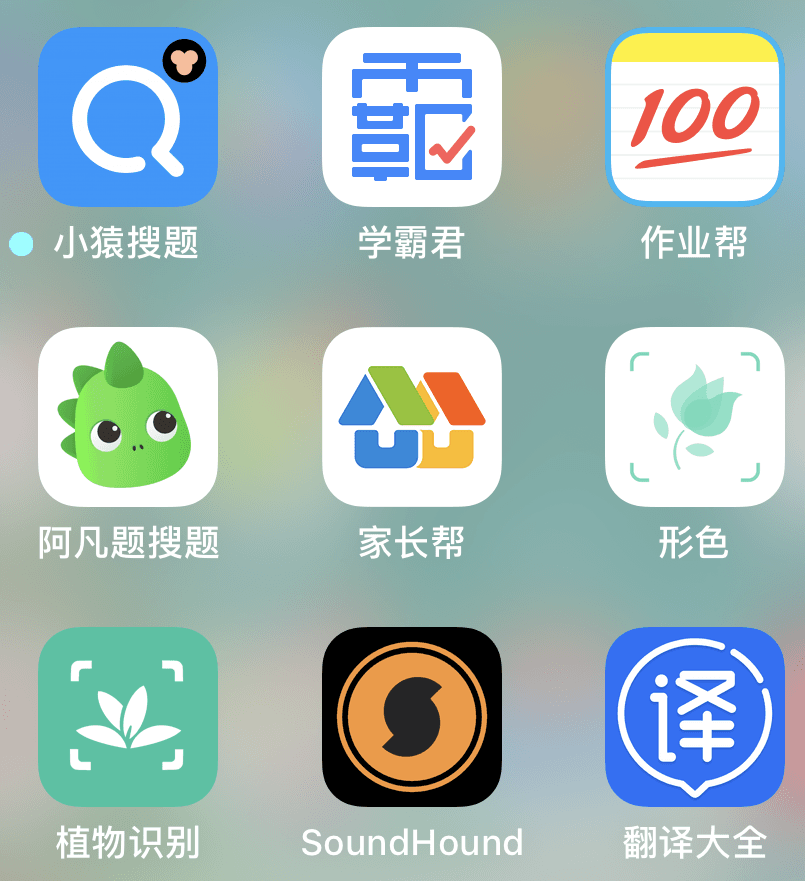
\includegraphics[scale=0.16]{search.png}
     	\caption{搜索$ App $}
     \end{figure}
     
  \end{frame} 

  \section{文献综述}
  \subsection{记忆模型与生理机制}
  \begin{frame}
  	  \begin{figure}
  	  	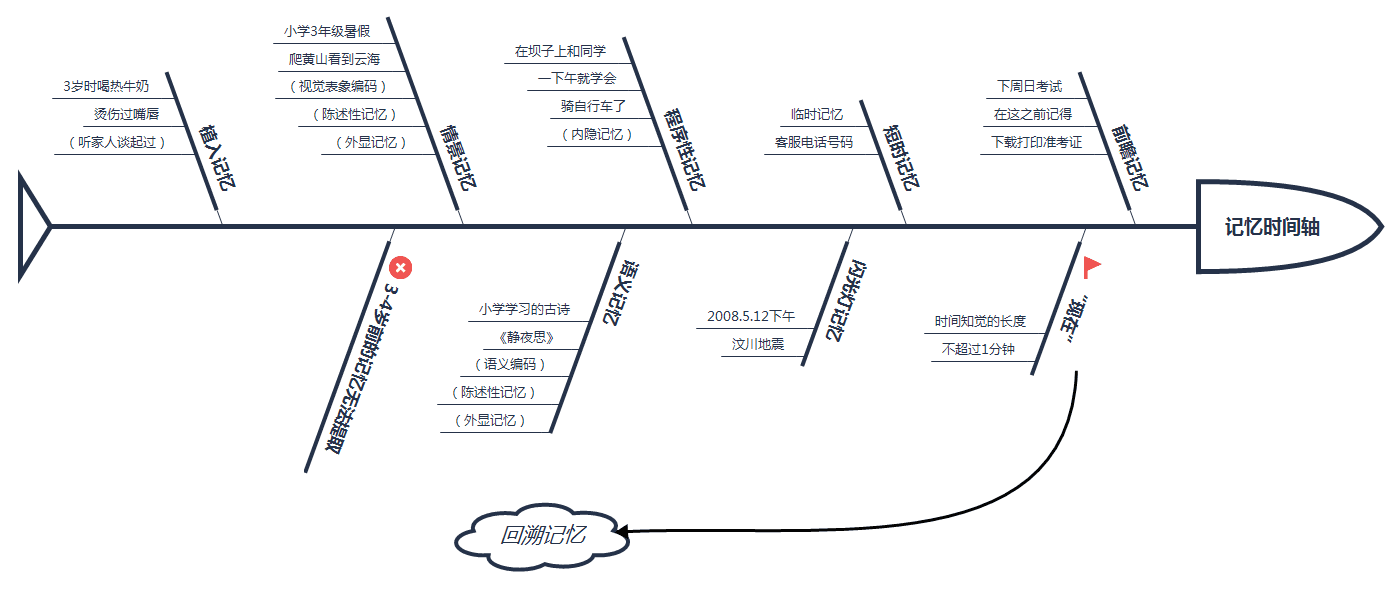
\includegraphics[scale=0.25]{timeaxis.png}
  	  	\caption{时间轴上的记忆类型}
  	  \end{figure}
  \end{frame}
  
  \subsubsection{记忆模型}
  \begin{frame}{记忆的模型}
        记忆虽然就是通过感觉获得信息,进行加工(将信息转换成可用的形式),组织存储的信息,并从存储中提取信息的过程。
        但它绝不是简单的对情景“拍照”,对语义的“笔录”,而是一个建构重塑的过程。
        \pause
        \begin{block}{能够触及记忆本质的两个记忆模型}
        	记忆多重存储模型\\
        	{\tiny (得到脑科学研究临床病例实证支持,确有短时记忆转入长时记忆障碍患者,模型表明大脑中确实存在不同类型的记忆,揭示了信息被编码、保持、提取的过程)}\\
            记忆加工水平模型\\
            {\tiny (可以更好的解释对信息进行不同水平的加工会产生不同记忆效果的现象,还能很好的解释自我参照效应(self-reference effect)可以增强记忆效果)}
        \end{block}
  \end{frame}
  
  \begin{frame}{记忆多重存储模型}
       \begin{figure}
       	\centering
       	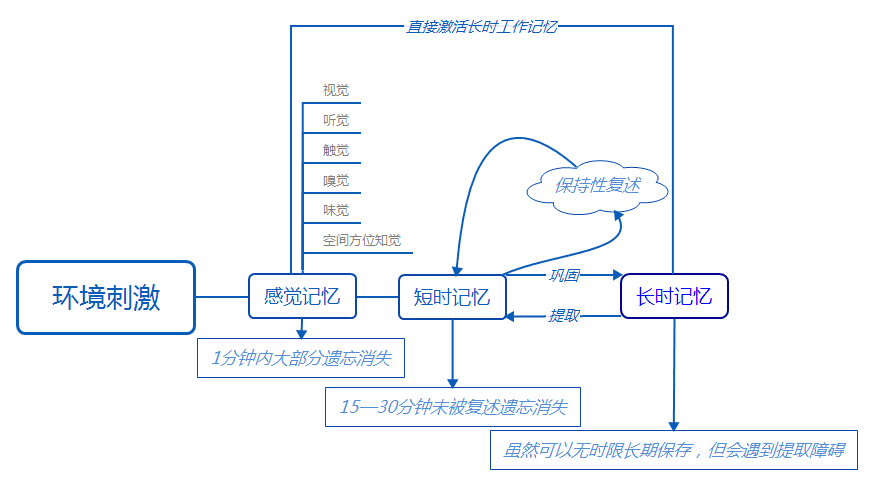
\includegraphics[scale=0.4]{记忆多重存储模型.png}
       \end{figure}
  \end{frame}
  
  \subsubsection{记忆生理机制}
  \begin{frame}{记忆生理机制}
     成人几乎所有部位的神经元是不能再生更新的,到是神经元的突触连接是在增加的,故而智力在不断发展。海马回中的齿状回,是成人能持续产生新神经元的少数几个区域之一。这个区域已经被证明是形成记忆的重要区域。\\
    \pause
    \begin{block}{记忆如何存储与存储在哪里?}
    	短时存储表现为神经递质的释放增加,长时存储表现为新突触的生成\\
    	(突触是一个神经元的轴突与另一个神经元的树突之间的狭窄间隙。)
    \end{block}
  \end{frame}
  
  \begin{frame}%{title}
       \begin{figure}[t]
       	\centering
        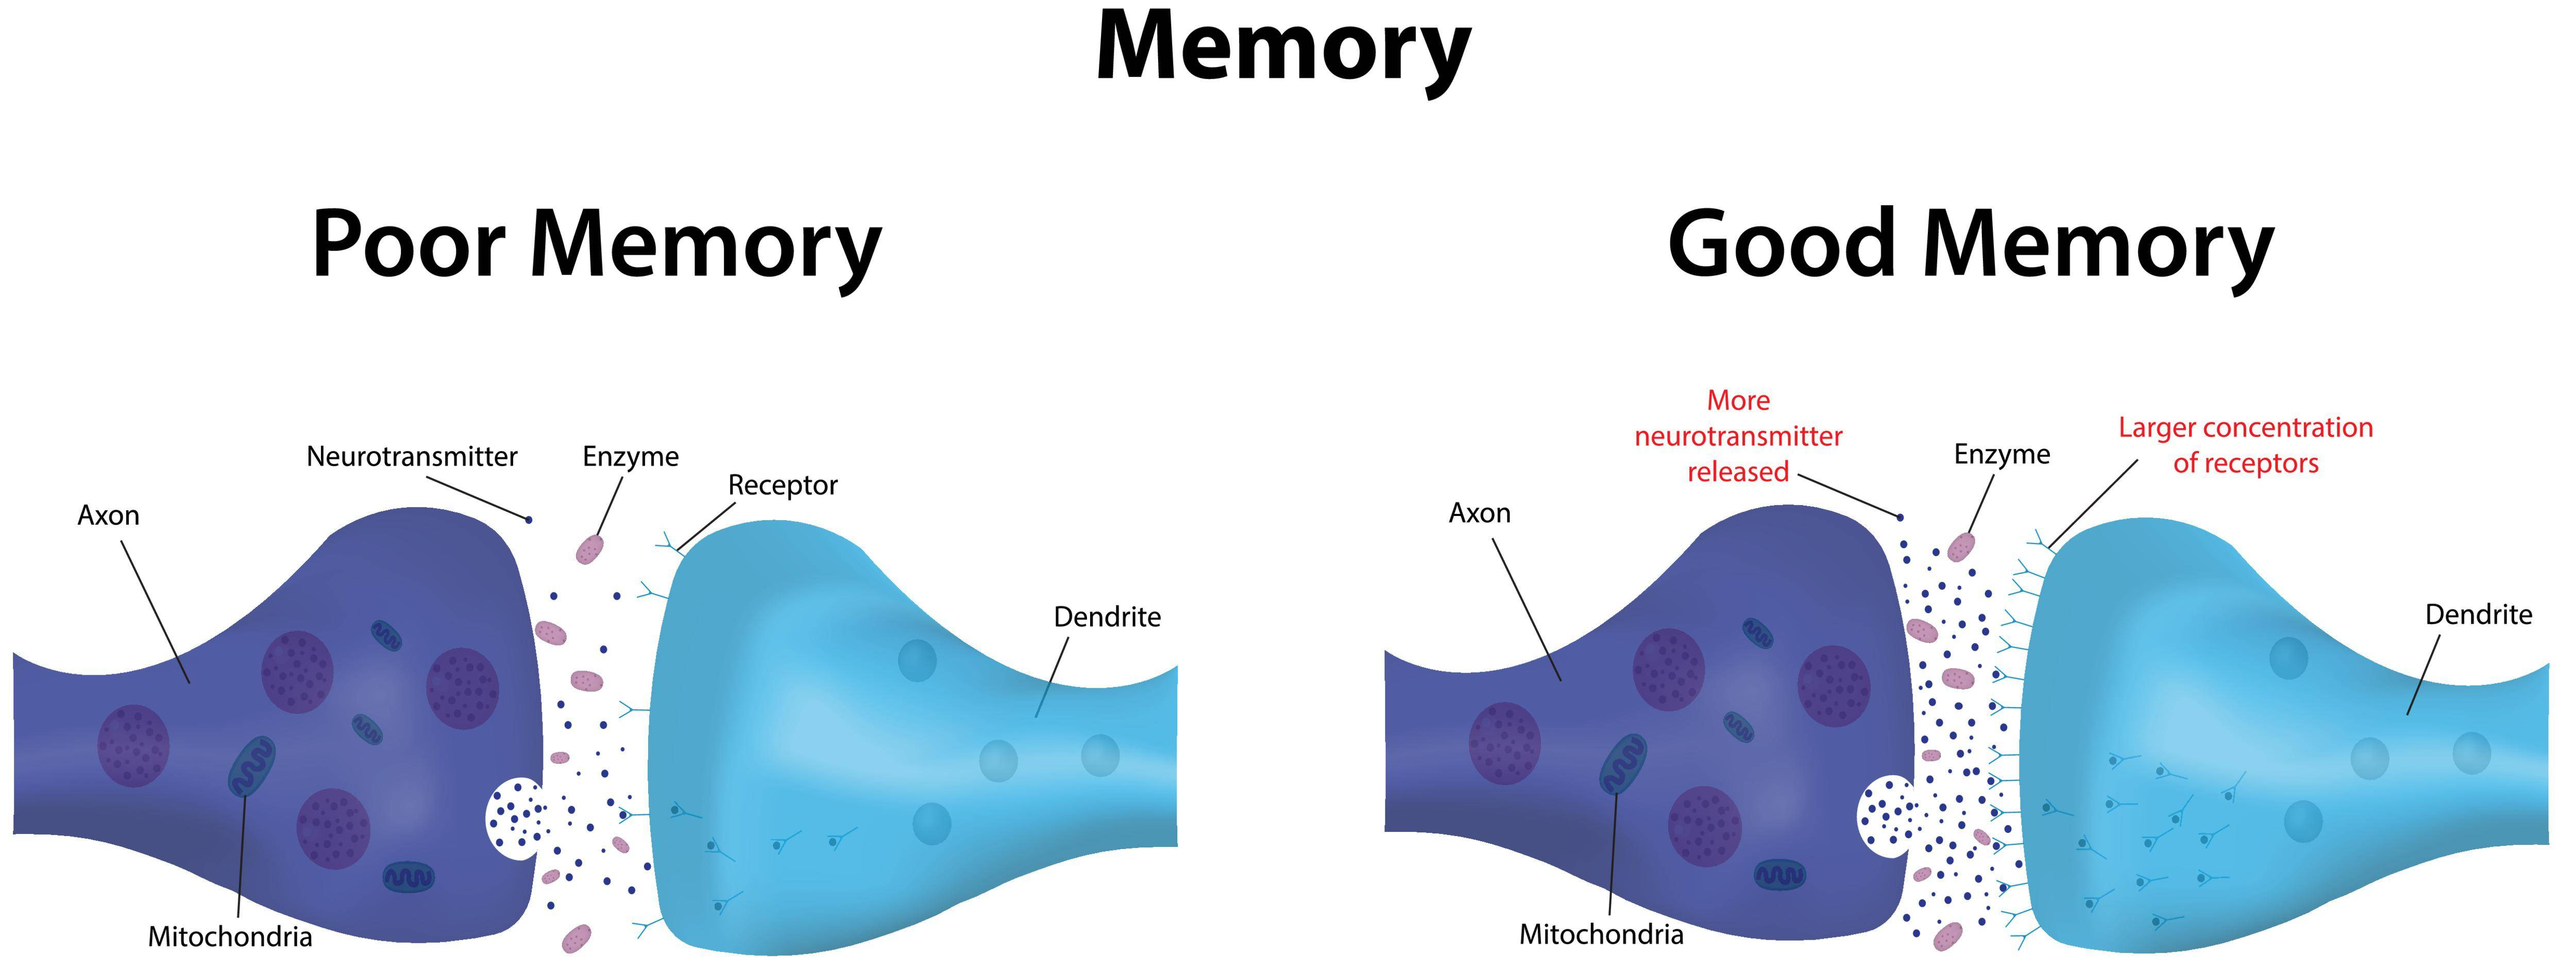
\includegraphics[scale=0.28]{model1.jpg}
        \caption{神经递质释放增加促成短时存储}
       \end{figure}
  \end{frame}

  \subsection{各种类型的记忆}
  \begin{frame}{工作记忆}
      工作记忆掌控着意识流与思维走向,它不只是简单地你记住了什么,而是你可以以怎样的效率干什么.\\
      工作记忆还包含诸如连接、转换等信息处理过程,仅凭短时记忆存储是无法实现的.\\
      \pause
      \begin{description}
      	\item[语音回路] 主要用于记住词的顺序,保持信息
      	\item[视觉空间模板] 主要用于加工视觉和空间信息(比如心理旋转)
      	\item[中央执行系统] 除了控制加工以外也有一定信息储存能力\\(调控中如果某一子系统需要,在调用其他子系统资源进行支援时用作为中转储存)
      \end{description}
  \end{frame}
  
  \begin{frame}{工作记忆模型}
  \begin{figure}[t]
  	\centering
  	\includegraphics[scale=0.3]{model2.jpg}
  	\caption{改进后的Baddeley工作记忆模型}
  \end{figure}
  \end{frame}
  
  \begin{frame}{长时记忆}
       \begin{itemize}
       	 \item 实验证实短时记忆和长时记忆遗忘的主要原因均是干扰(曾一度认为短时记忆遗忘的主要原因是消退)
       	 \item “干扰抑制回忆,提取诱发遗忘”这个研究结果对数学教学很有意义
       	 \item 长时记忆既包含陈述性记忆,还包含程序性记忆
       	 \item 长时记忆的组织方式与因特网类似,储存的知识具有语义网络的结构,语义相关的都会产生超链接
       	 \item 通过训练和长期实践应用特定领域的记忆技能可以形成长时工作记忆,记忆中的专家效应
       \end{itemize}
  \end{frame}
  
  \begin{frame}{记忆研究新领域}
      \begin{description}
      	\item[元记忆] 监控个体自身记忆对象和进程的记忆
      	\item[自传体记忆] 伴有情绪感情色彩,构建自身基模之上,附着个人个性信息的记忆
      	\item[内隐记忆] 无需意识参与的记忆
      	\item[前瞻记忆] 指向未来带有计划性的记忆
      	\item[错误记忆] 被暗示,产生偏差,被动植入等导致的有悖事实的记忆
      \end{description}
  \end{frame}
  
  
  \section{研究方法与框架}
  \subsection{研究方法}
  \begin{frame}{研究方法}
     \begin{block}{文献研究}
     	对于脑科学和心理学,自身专业知识和实验条件均存在短板,主要通过阅读学习相关学术文献,试图将架构更底层,具备一般性的前沿研究成果运用到中学数学课堂教学中
     \end{block}
     \pause
     \begin{block}{案例研究}
     	对中学数学课堂教学中积累的素材、典型案例、经验做法回顾反思,收集有助于记忆的教学素材,提炼有效的经验做法
     \end{block}
  \end{frame}
  
  \begin{frame}{研究方法}
      \begin{block}{行动研究}
    	对已有一定教学积累,感觉有效的记忆策略,且在以往教学中得到部分验证的想法、课例,展开行动研究。重新思考教学计划、展开行动、多方面观察教学实效,在此基础上进行反思归纳。更新想法,再修订,再展开新一轮行动研究
    \end{block}
    \pause
    \begin{block}{调查研究}
  	    尝试验证文献研究中结论有出入、观点有分歧的问题;了解元记忆的监测与控制水平;验证之前一些仅凭经验归纳提炼的数学记忆策略
    \end{block}
\end{frame}
  
  \subsection{研究框架}
  \begin{frame}{研究框架}
      \begin{figure}[t]
      	%\raggedleft
      	%\centering
      	\raggedright
      	%\raggedbottom
      	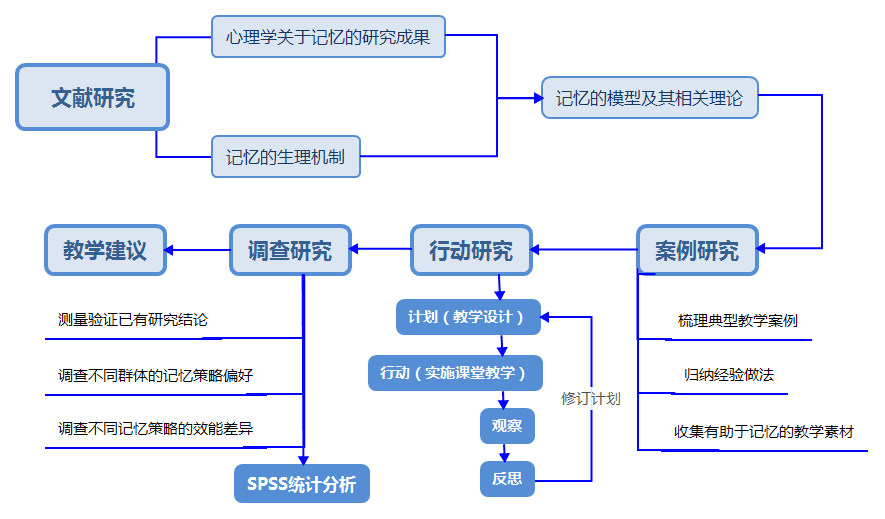
\includegraphics[scale=0.35]{researchframe.png}
      	%\caption{研究框架}
      \end{figure}
  \end{frame}
   %\part{第一节}
   %\begin{frame}{研究目的}
   %   \partpage
   %    请插入图片
   %   \begin{figure}[b]
   %      \raggedleft
   %      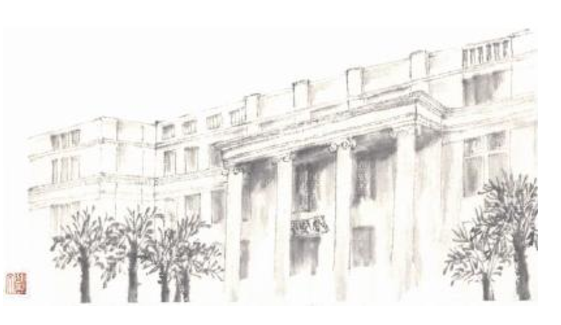
\includegraphics[scale=0.4]{WSbuilding.pdf}	
   %      \caption{}
   %   \end{figure}
   %\end{frame}
    \section{研究过程}
    \subsection{案例研究与行动研究}
    \subsubsection{提高工作记忆在数学活动中效率的策略}
       \begin{frame}{提高工作记忆活动效率的策略}
          \begin{columns}
          	\column{0.7\textwidth}
          	  \begin{block}{提高信息块(chunks)的质量}
          	  	$ x^3+y^3+z^3-3xyz=(x+y+z)(x^2+y^2+z^2-xy-yz-zx) $\\
          	  	$ \sum x^3-3xyz=(\sum x)(\sum x^2-\sum xy) $
          	  \end{block}
              \pause
              \begin{block}{优化算法减轻信息块调用负荷}
              	$ 74\times 76\longrightarrow\overline{7\times 8} \quad\overline{4\times6}\longrightarrow\overline{5624} $
              \end{block}
              \pause
              \begin{block}{发展长时工作记忆,形成专家记忆优势效应}
              	Basel问题$ 1+\frac{1}{4}+\frac{1}{9} \cdots +\frac{1}{k^2} +\cdots=\frac{\pi^2}{6} $\\
              	欧拉计算时毫不费力,就像人呼吸或者鹰在风中保持平衡一样——物理学家阿拉果(法)
              \end{block}
          	\column{0.25\textwidth}
          	\pause
          	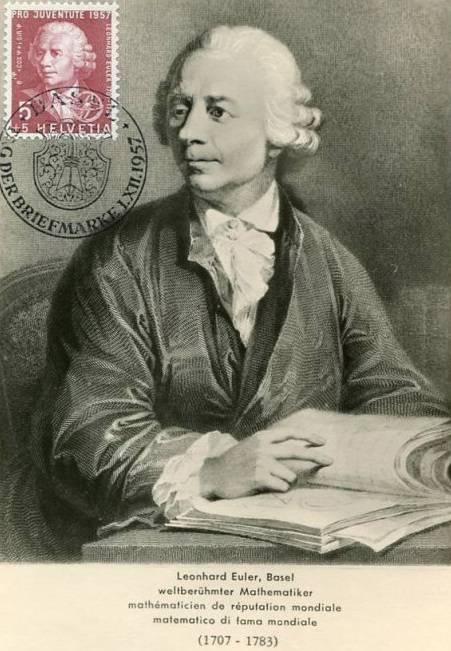
\includegraphics[scale=0.6]{EULER1.jpg}
          \end{columns}
       \end{frame}
   
    \subsubsection{提升数学活动中长时记忆效果的策略}
        \begin{frame}{提升长时记忆效果的策略}
           \begin{block}{及时回顾与形式丰富的回忆}
           	$ \sin \alpha=\frac{y}{r}=\frac{y}{\sqrt{x^2+y^2}}=\frac{1}{\csc \alpha}=\pm \frac{1}{\sqrt{1+\cot^2\alpha}} $
           	
           	$=\tan \alpha \cos \alpha=\frac{\cos \alpha}{\cot \alpha}=\pm \sqrt{1-cos^2\alpha} $
           
            $ =\cos (\frac{\pi}{2}-\alpha) =-\cos (\frac{\pi}{2}+\alpha) =\sin (\pi-\alpha)=-\sin (\pi+\alpha)  $
            
            $ =-\cos (\frac{3\pi}{2}-\alpha) =\cos (\frac{3\pi}{2}+\alpha) =-\sin (-\alpha)=\sin (2k\pi+\alpha)  $
            
            $ =\sin(\alpha-\beta) \cos \beta + \cos (\alpha-\beta) \sin \beta  =\sin(\alpha+\beta) \cos \beta - \cos (\alpha+\beta) \sin \beta$
            
            $=\sin(\frac{\alpha+\beta}{2})cos(\frac{\alpha-\beta}{2})+\cos(\frac{\alpha+\beta}{2})\sin(\frac{\alpha-\beta}{2}) $
            
            $=\sin(\frac{\beta+\alpha}{2})cos(\frac{\beta-\alpha}{2})-\cos(\frac{\beta+\alpha}{2})\sin(\frac{\beta-\alpha}{2}) $ 
            
            $=2\sin\frac{\alpha}{2} \cos \frac{\alpha}{2}=(\sin\frac{\alpha}{2}+\cos\frac{\alpha}{2})^2-1=1-(\sin\frac{\alpha}{2}+\cos\frac{\alpha}{2})^2=\frac{2\tan\frac{\alpha}{2}}{1+\tan^2\frac{\alpha}{2}} $
            
            $ =\frac{2}{\tan\frac{\alpha}{2}+\cot\frac{\alpha}{2}}=\pm \sqrt{\frac{1-\cos2\alpha}{2}}=3\sin\frac{\alpha}{3}-4sin^3\frac{\alpha}{3}$
            
            $=\sqrt{2}\sin(\alpha+\frac{\pi}{4})-\cos\alpha=\cdots $
           \end{block}
        \end{frame}
    
        \begin{frame}{提升长时记忆效果的策略}
        \begin{block}{优化编码方式深度加工记忆信息}
        	\begin{figure}
        		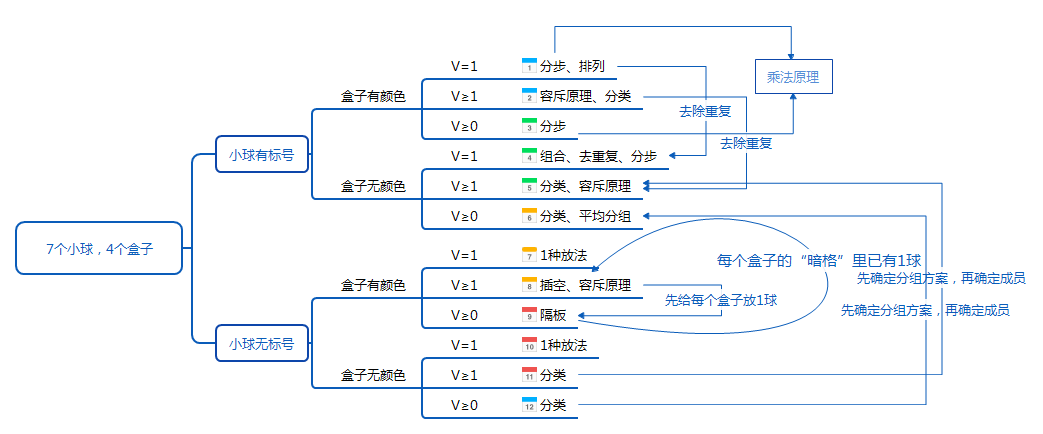
\includegraphics[scale=0.33]{combination.png}
        		\caption{计数问题结构框架与计数技巧方法思维导图}
        	\end{figure}
        \end{block}
        \end{frame}
        
        \begin{frame}{提升长时记忆效果的策略}
           \begin{block}{构建自己的联系丰富的数学知识网络}
           自己构建体系的记忆效果远远优于别人告诉我的同样内容.把记忆的东西与大脑中原有的东西联系起来,这种联系的神经通路越多,对记忆对象的描述就越全面,记忆对象会更加鲜活.	
           \end{block}
           \pause
           数学知识网络中的各种联系
           \begin{itemize}
           	\item 可以加深我们对知识的理解,从而使得减轻记忆负担,巩固记忆持效性 
           	\item 有利于通性通法的提炼,从而使得记忆提取线索更为精准,便于存储信息的检索、回忆、再现
           	\item 有利于联想、发散性思维和创造性思维
           \end{itemize}
        \end{frame}
        
        \begin{frame}{提升长时记忆效果的策略}
        对自传体记忆的研究表明自身知识网络的构建方式决定了记忆水平.记忆存储的信息不止知识与事实,还包含个人体验、感情色彩、情绪状态以及时空上的参照点等信息.把知识绑定自己的积极体验,主动建构知识网络,使之成为自传体记忆的一部分\\
        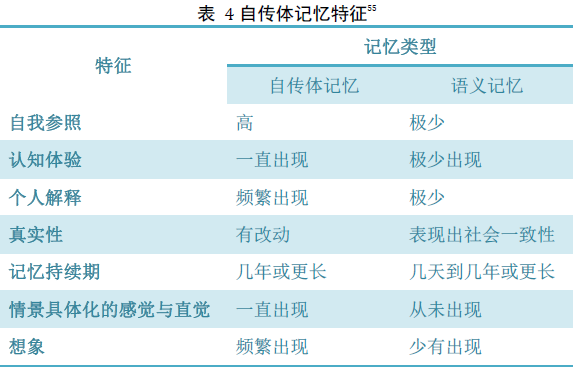
\includegraphics[scale=0.5]{autobiography1.png}
        \end{frame}
        
        \begin{frame}{提升长时记忆效果的策略}
        \begin{block}{视觉技能发掘长时记忆潜力}
        	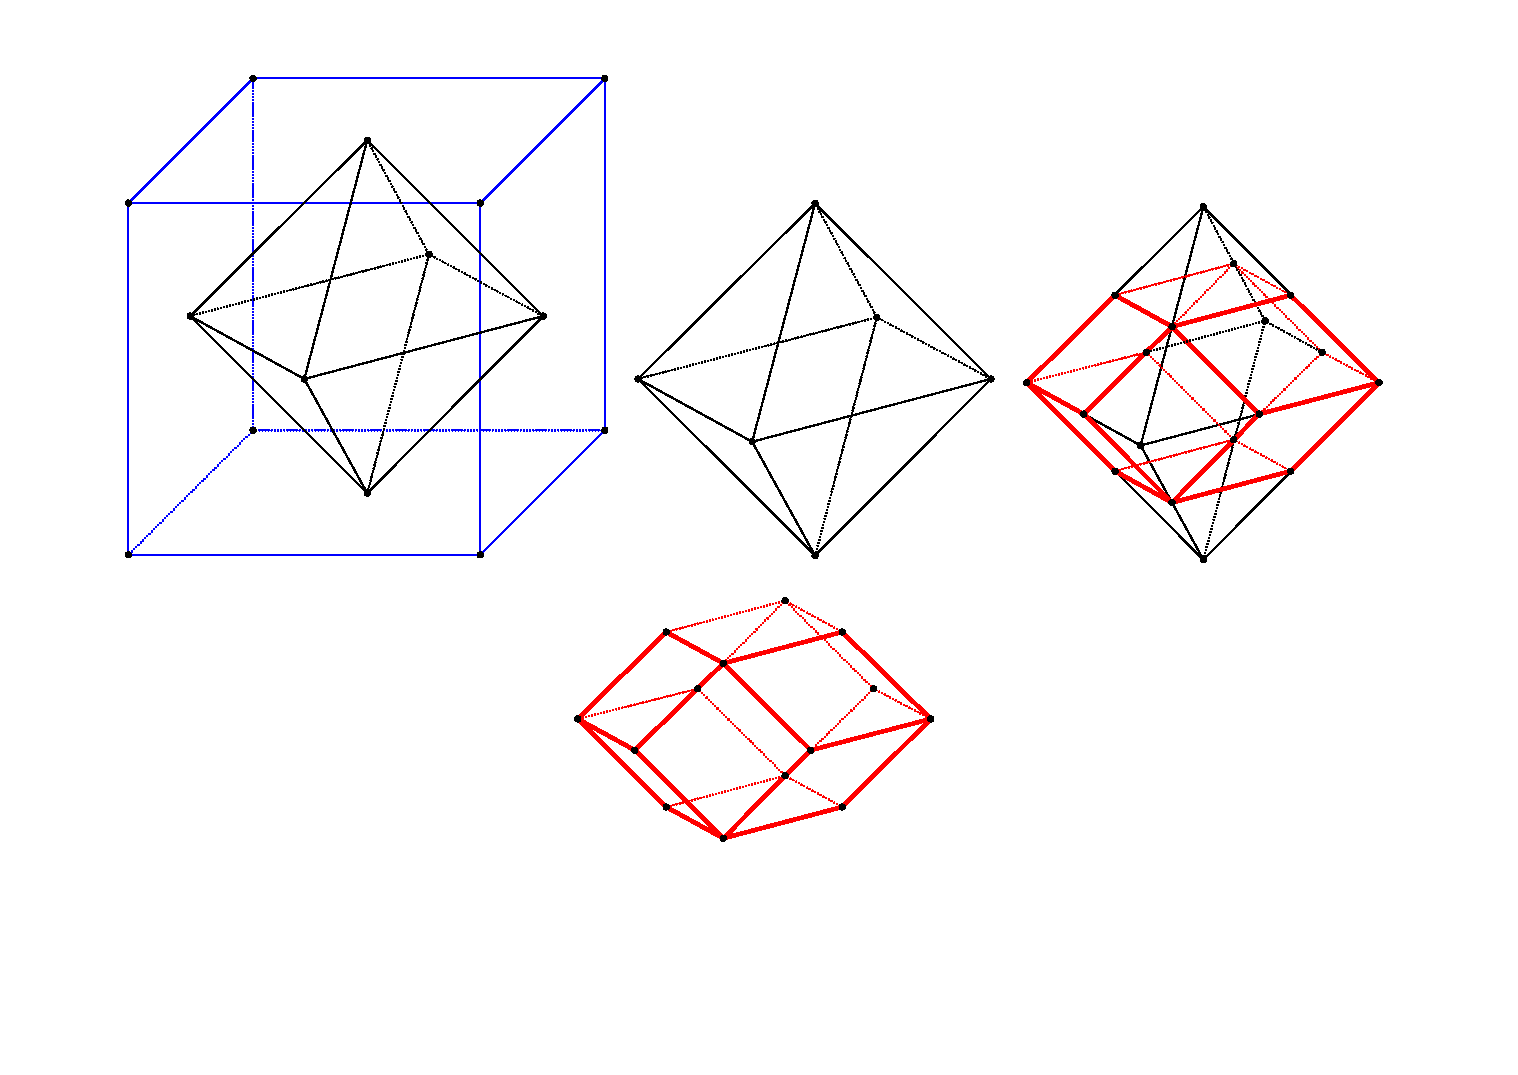
\includegraphics[scale=0.32]{prism.pdf}
        \end{block}
        \end{frame}
        
        \begin{frame}{提升长时记忆效果的策略}
        \begin{block}{令数学记忆生动起来的队列阵形变换}
        	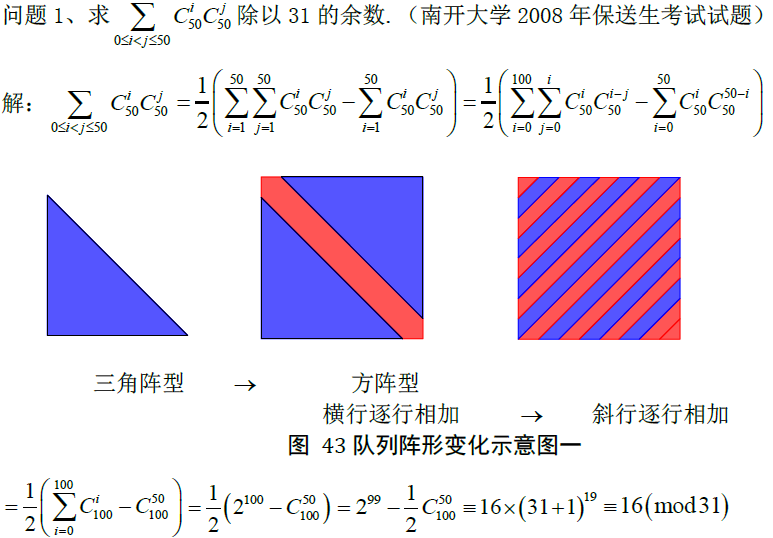
\includegraphics[scale=0.4]{array.png}
        \end{block}
        \end{frame}
    
    \subsubsection{在数学活动中发挥多重记忆系统合力的策略}
         \begin{frame}{发挥多重记忆系统合力的策略}
           \begin{block}{巧设数学活动——寓教于乐中的内隐记忆}
           	演绎推理的方式,记忆的对象不仅有公式,也有蕴含其中的数学思想,它的学习一般需要有意注意,相应的记忆也是外显记忆;\\
           	而操作摸索的过程中更多的是无意注意,摸索得到的结论不经意间已留下深刻印象,相
           	应的记忆是内隐记忆.内隐记忆存储的信息丰富生动完整,能保持的时间更长,在迁移提取时比外显记忆更稳定.\\
            $\bigstar $\quad	两种方式协同进行时学习效果最好
           \end{block}
           \pause
           \begin{block}{规范流程与提炼靶事件编码对前瞻记忆的促进}
           	  \begin{itemize}
           	   \item 规范严谨的程式让前瞻记忆成为无需意识的自动激活加工
           	   \item 提高靶事件的编码质量降低前瞻记忆对注意分配的要求
             \end{itemize}
           \end{block}
         \end{frame}
     
    \subsection{调查研究}
    \subsubsection{问卷设计}
    \begin{frame}{问卷}
         \begin{columns}
         	\column{0.45\textwidth}
         	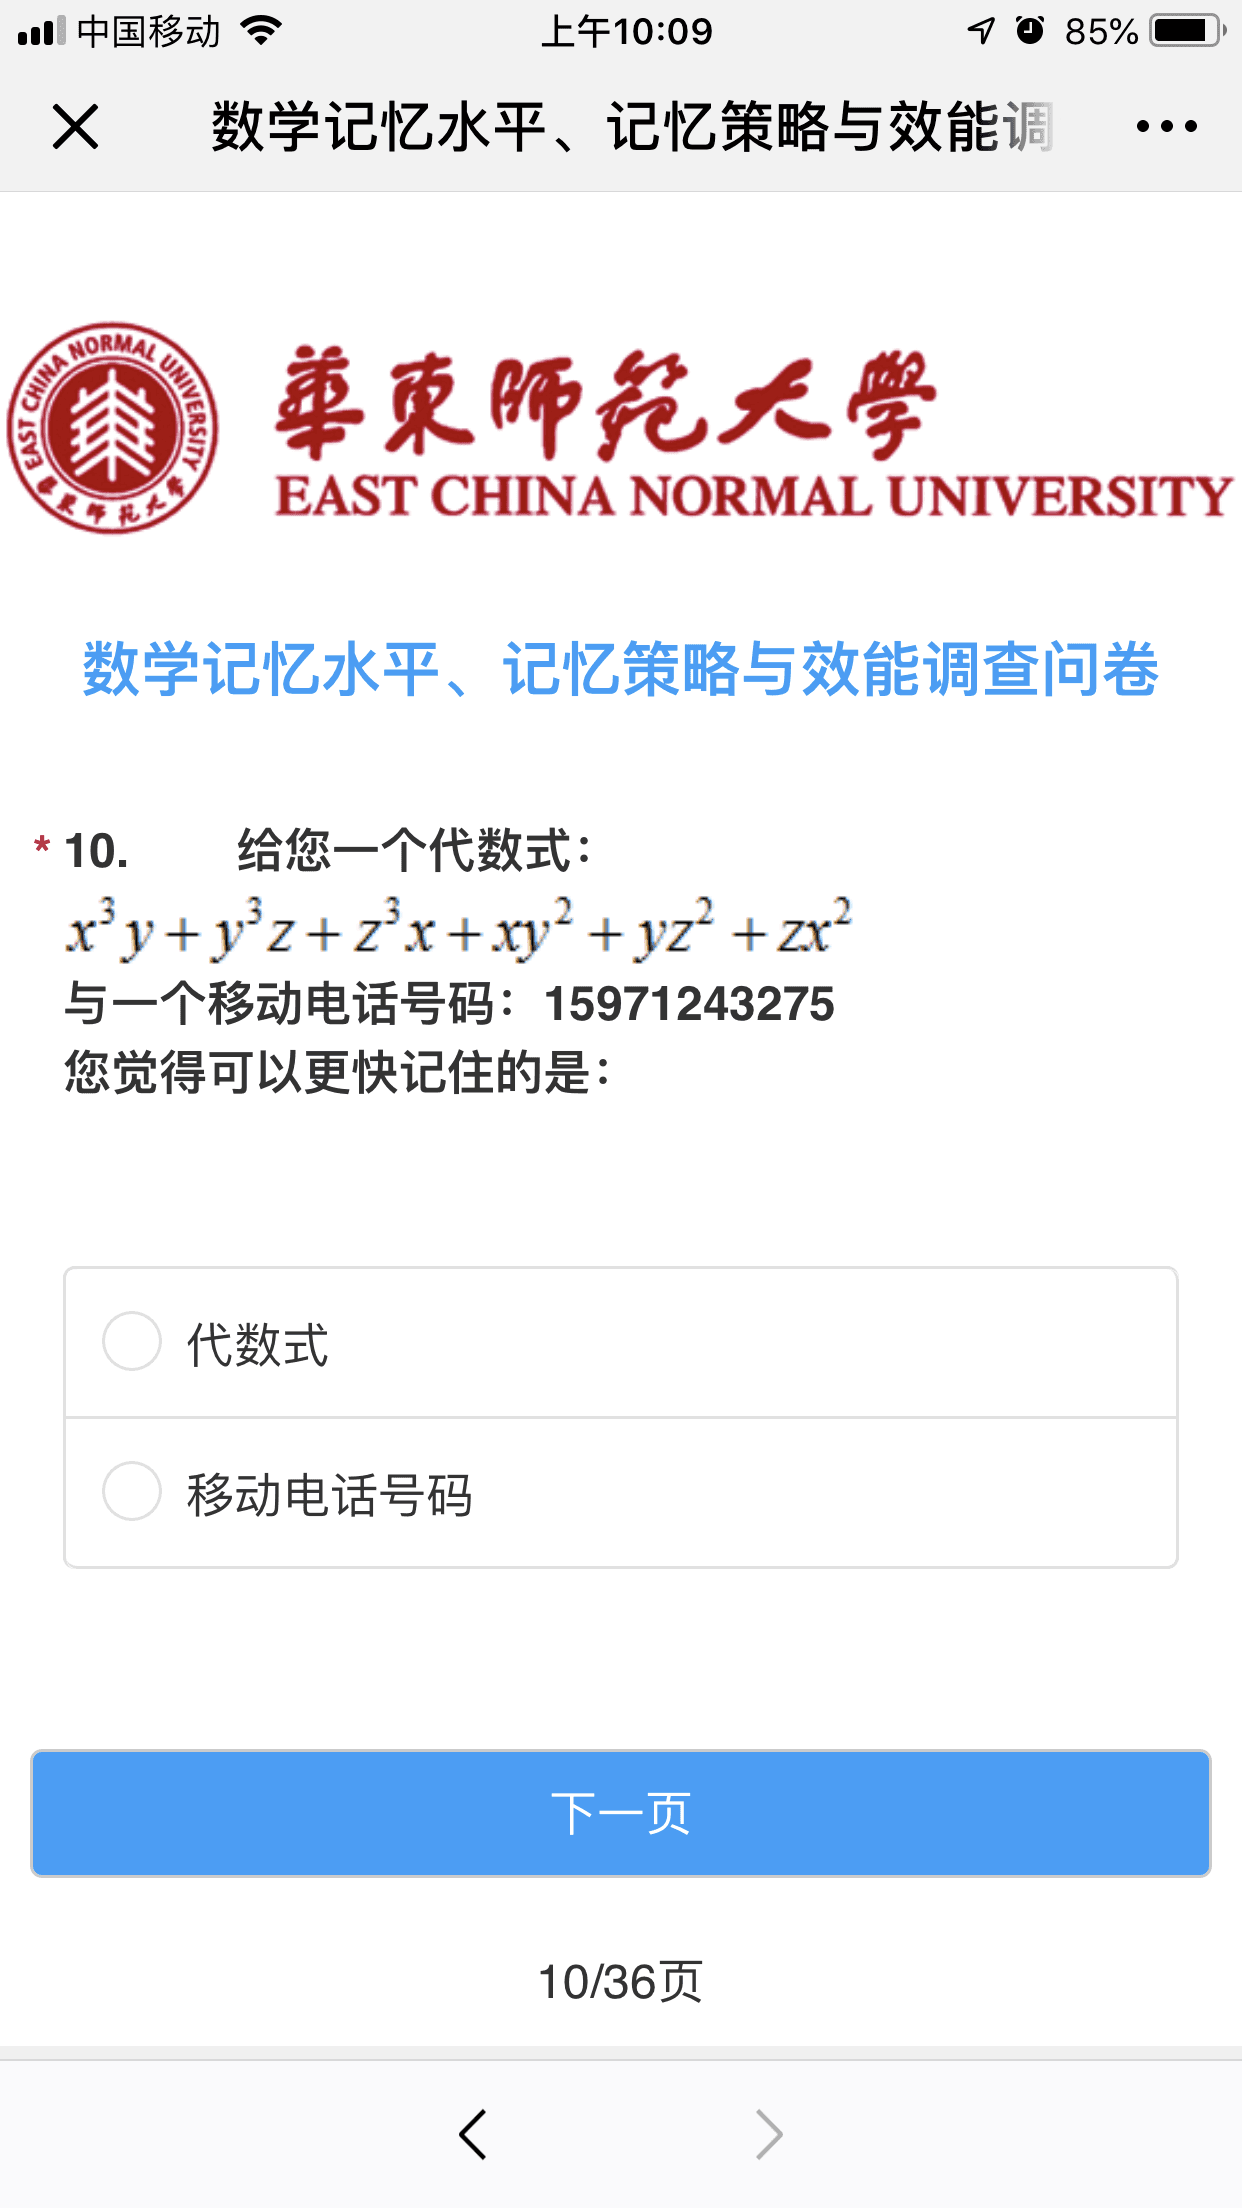
\includegraphics[scale=0.09]{test10.png}
         
            \column{0.45\textwidth}
        	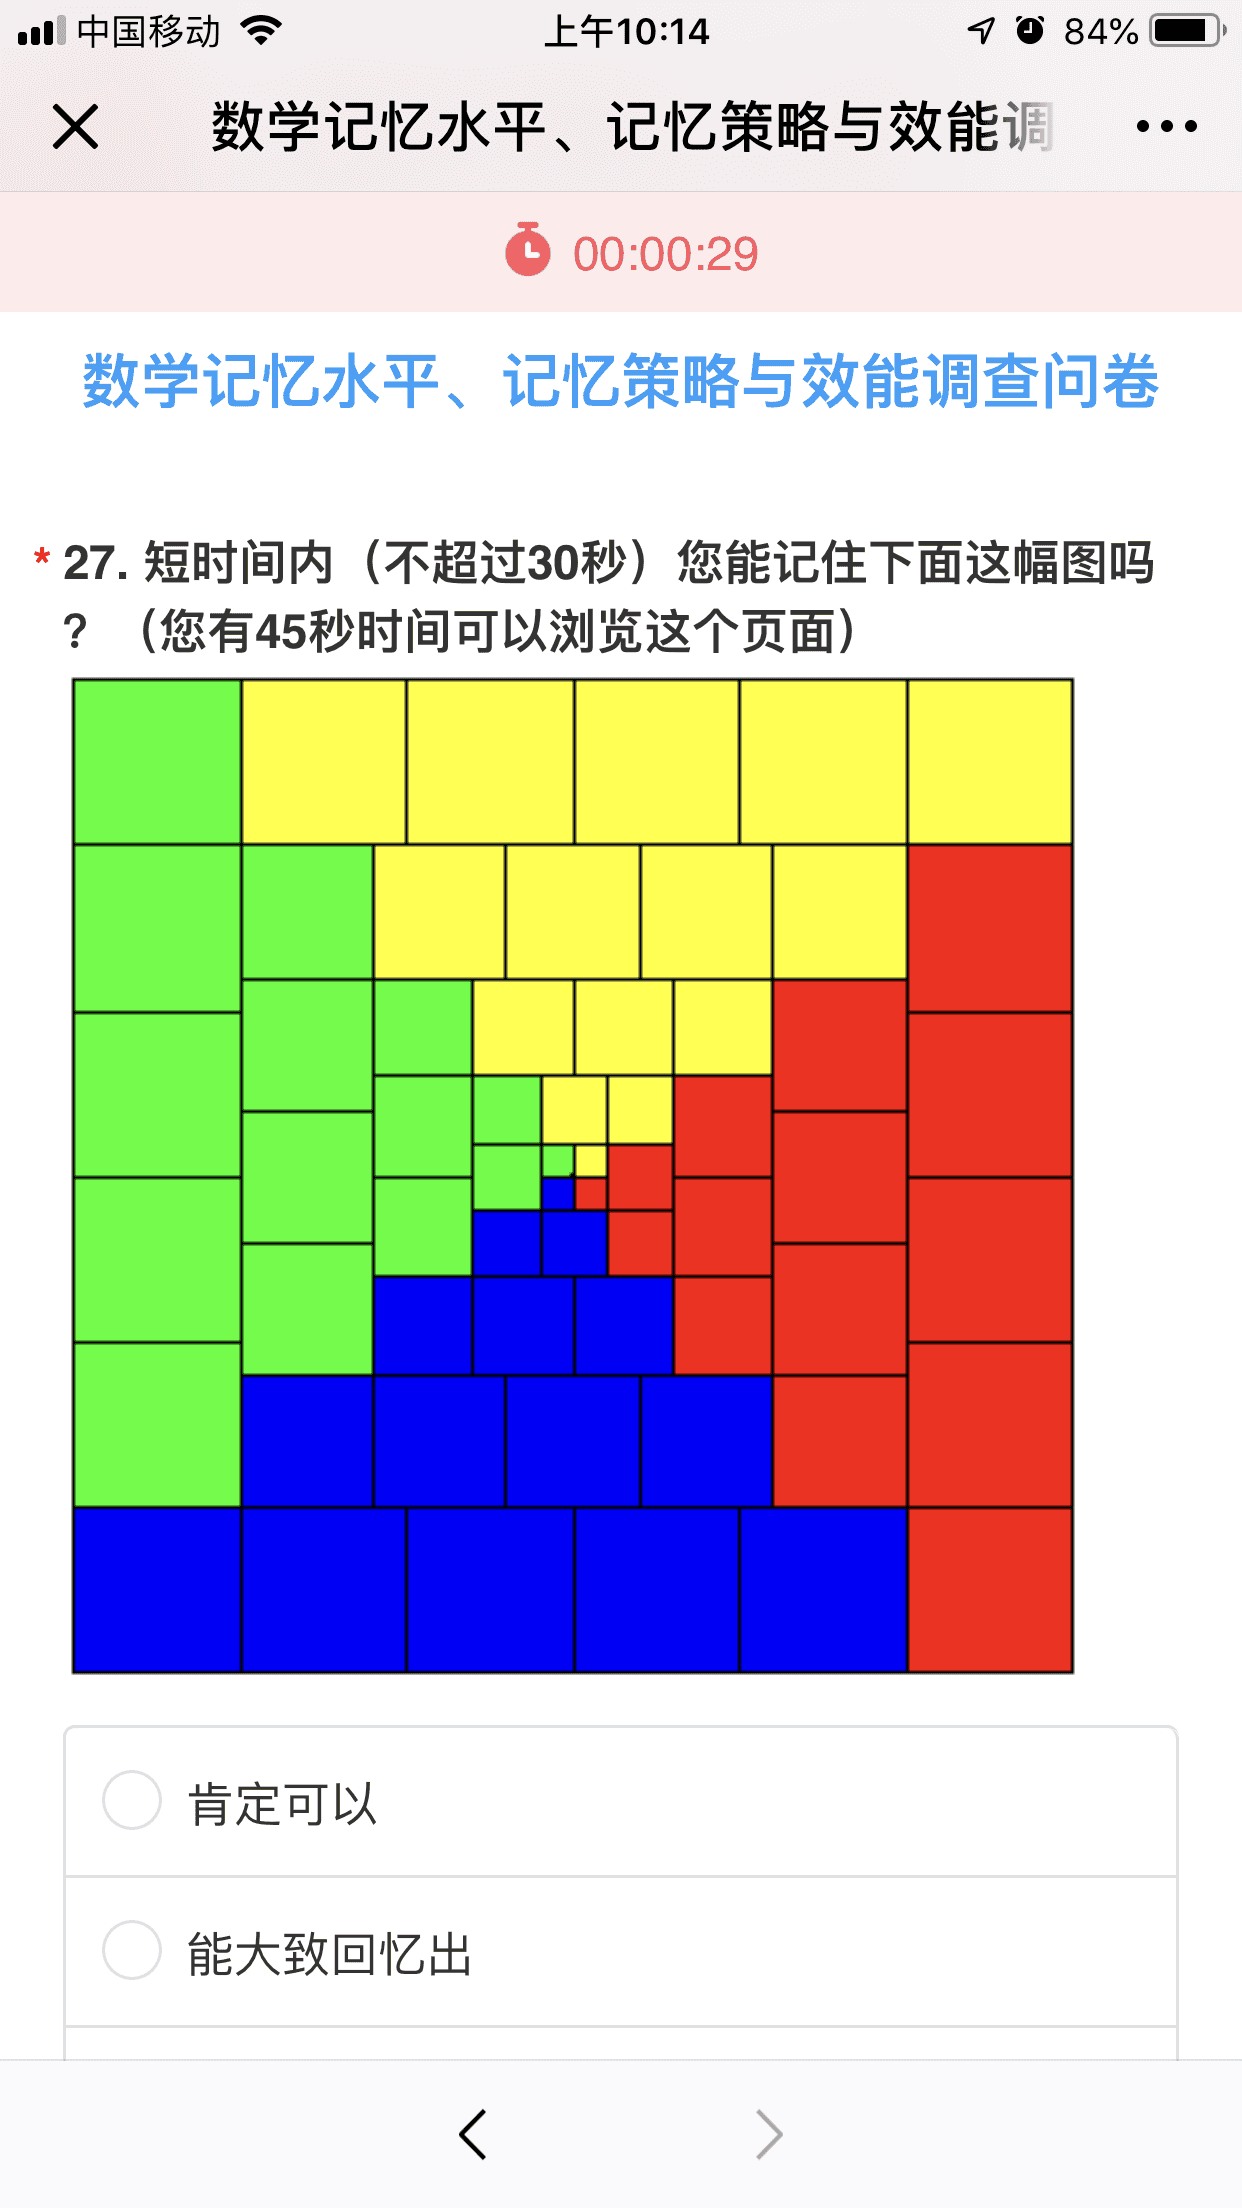
\includegraphics[scale=0.09]{test27.png}
        \end{columns}            
    \end{frame}
    
    \subsubsection{数据分析}
    \begin{frame}{统计检验方法选择}
        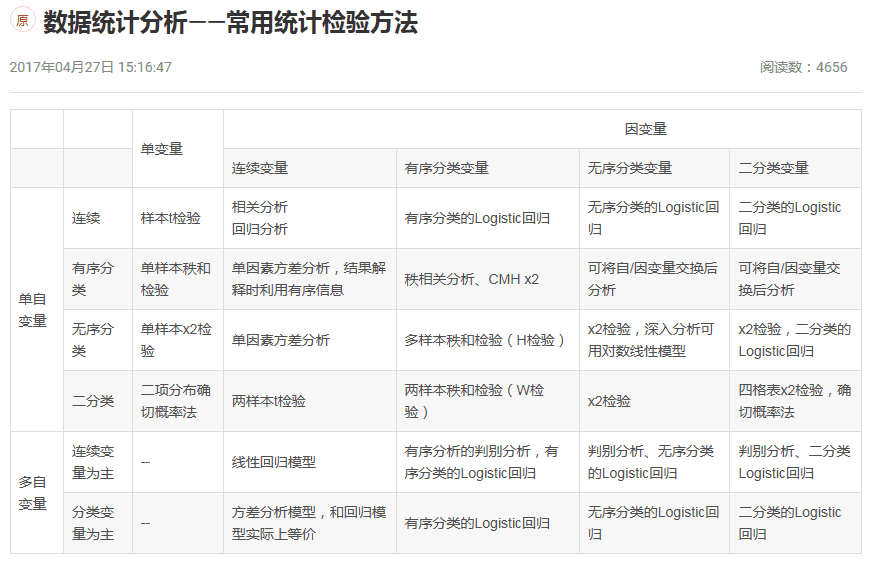
\includegraphics[scale=0.47]{statisticaltest.png}
    \end{frame}

    \begin{frame}{短时记忆容量}
    \begin{columns}
    	\column{0.35\textwidth}
    	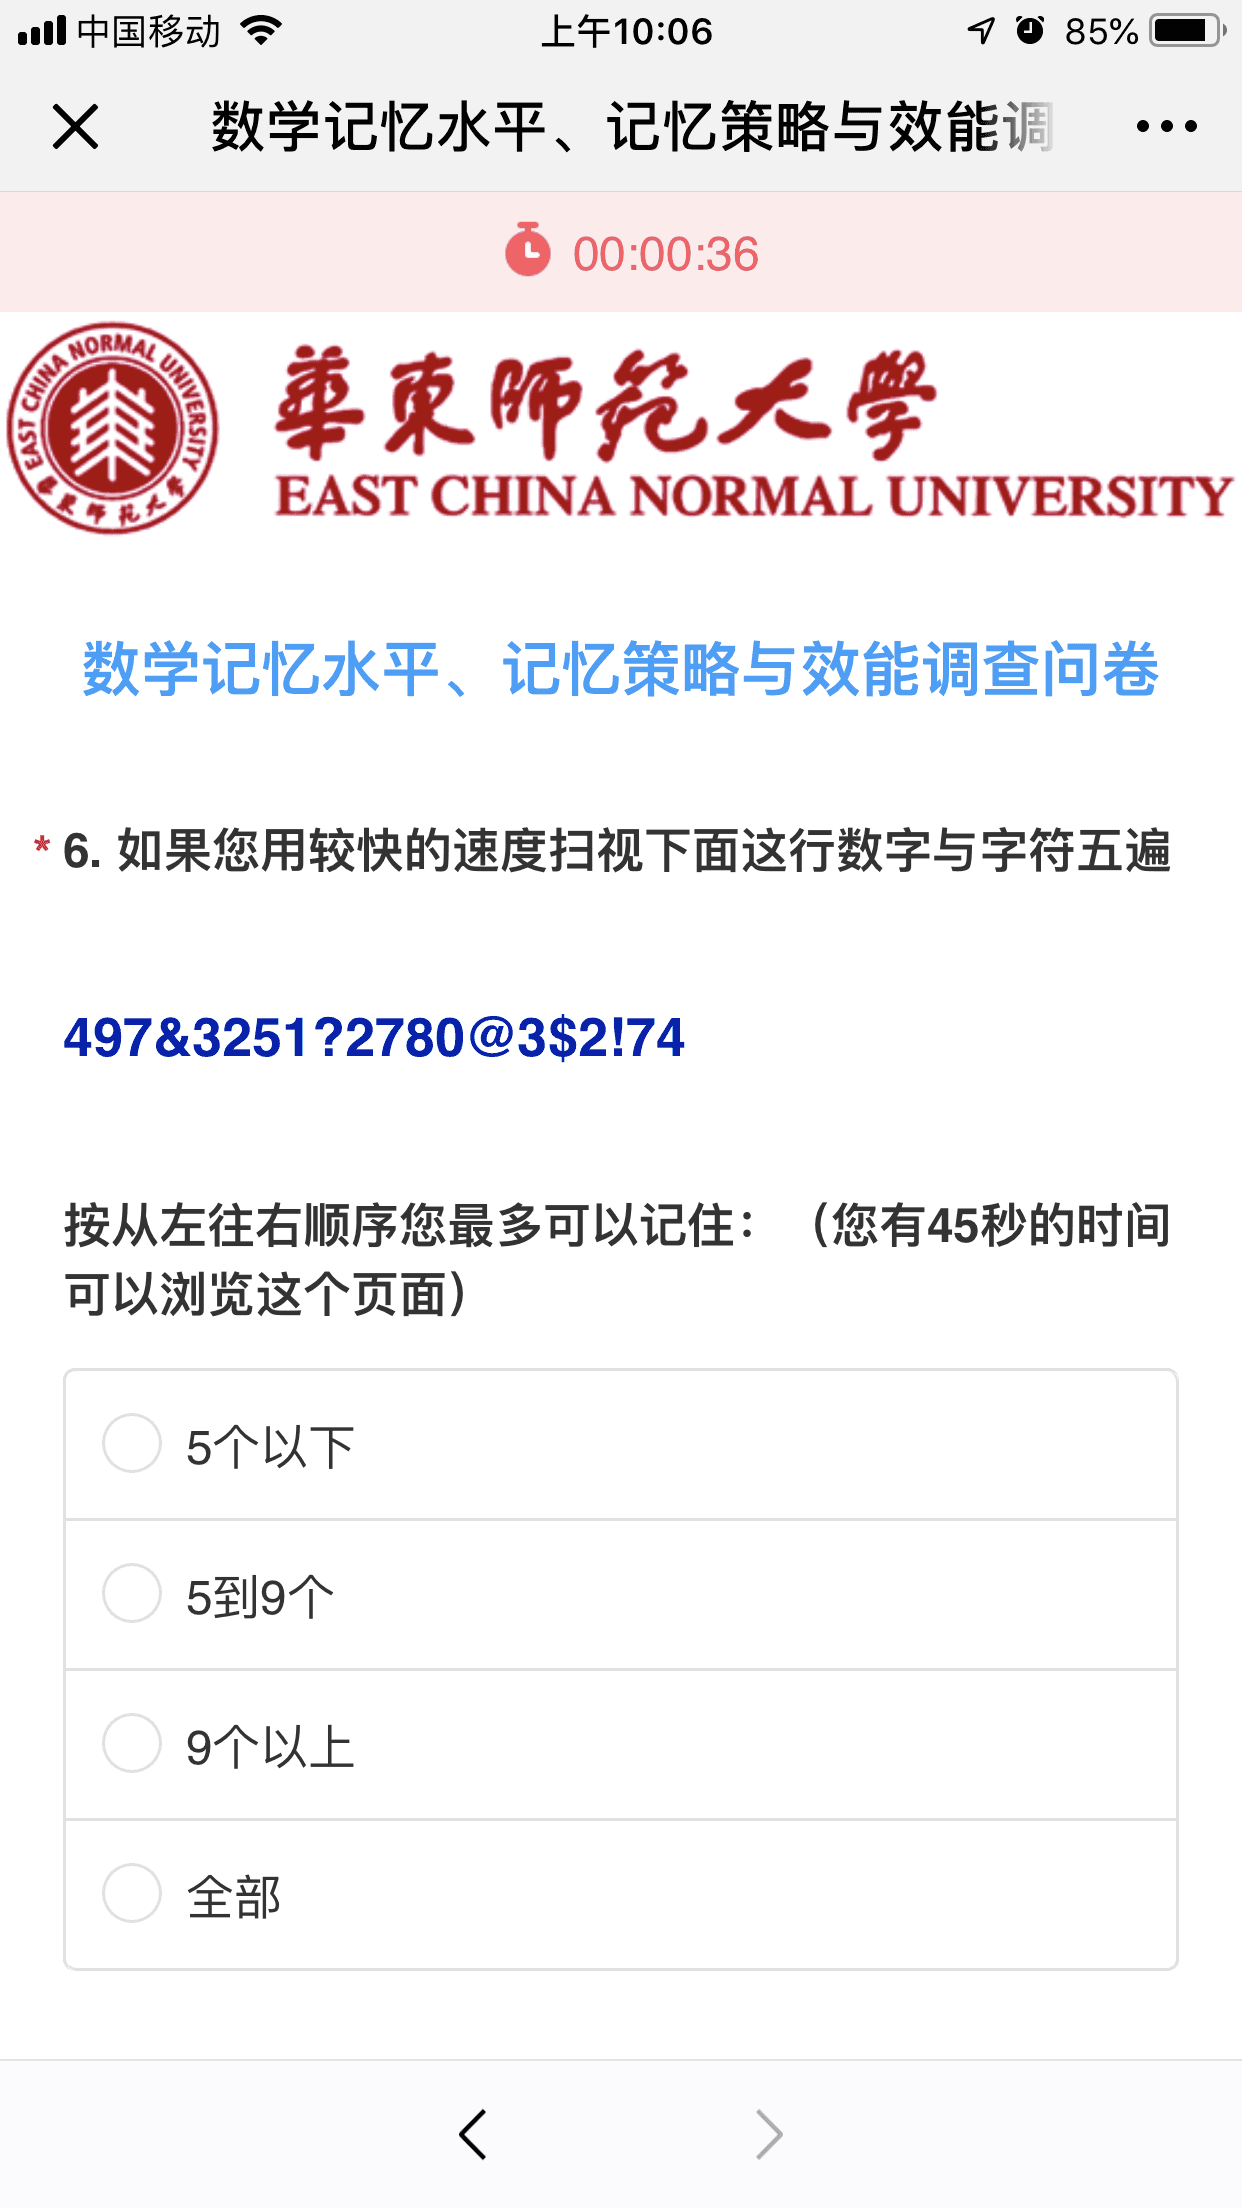
\includegraphics[scale=0.08]{test6.png}\\
    	\scriptsize{15秒后才可以点下一页,}\\
    	\scriptsize{45秒后自动跳往下一页}
    	\column{0.35\textwidth}
    	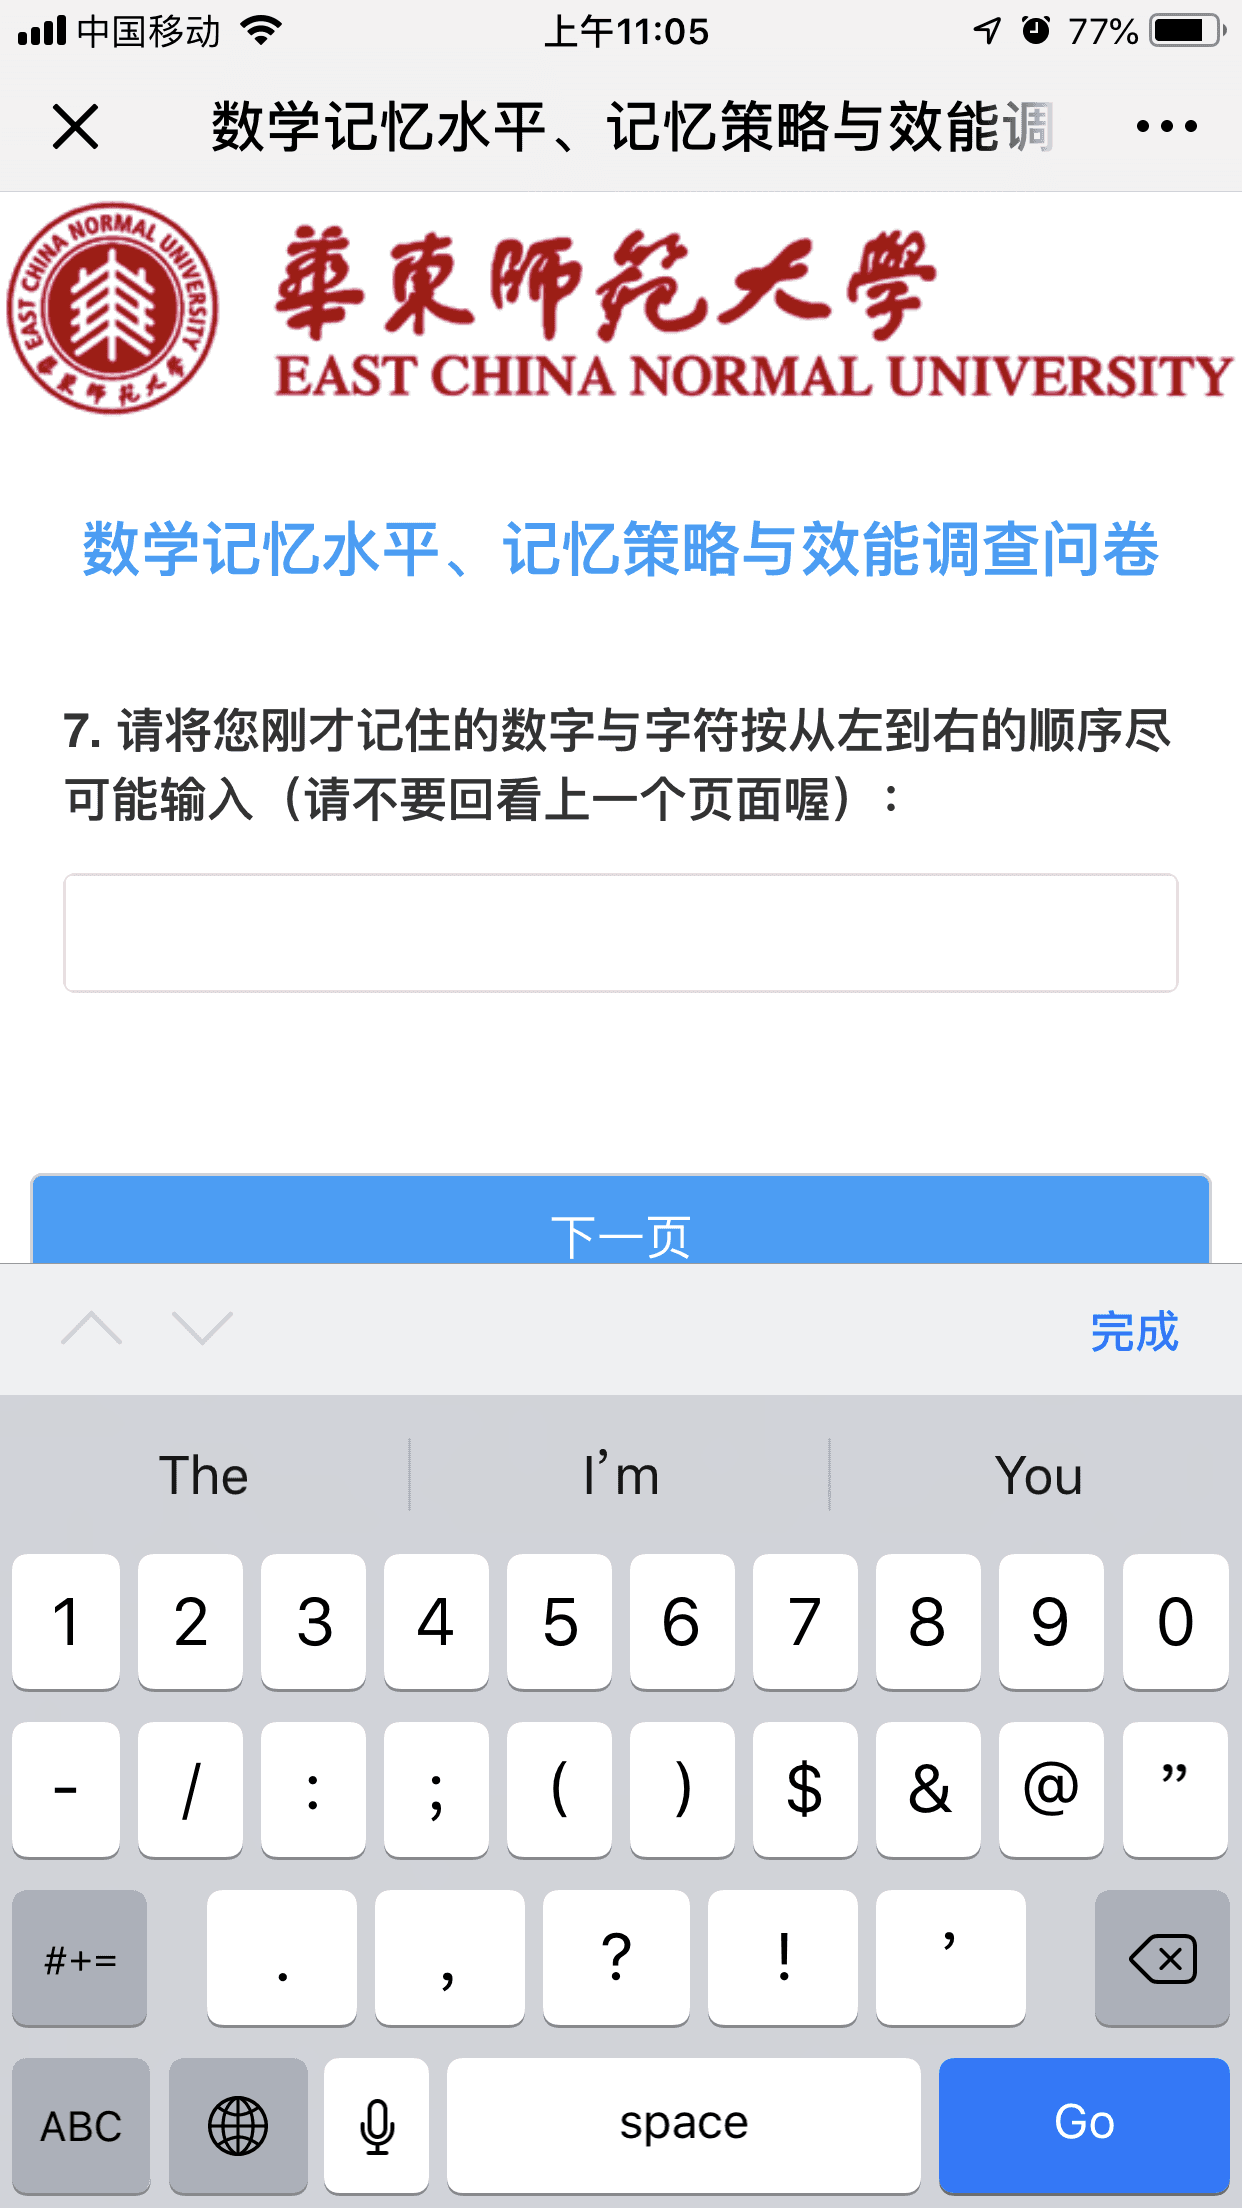
\includegraphics[scale=0.08]{test7.png}\\
    	\scriptsize {要输入的数字与字符在同一}\\
    	\scriptsize {软键盘,减小操作影响}
    	\column{0.3\textwidth}
    	\begin{block}{验证结论}
    		短时记忆容量的平均值为:$ 6.596 $ 个字符
    	\end{block}    	
    \end{columns}            
    \end{frame}
    
    \begin{frame}{元记忆}
          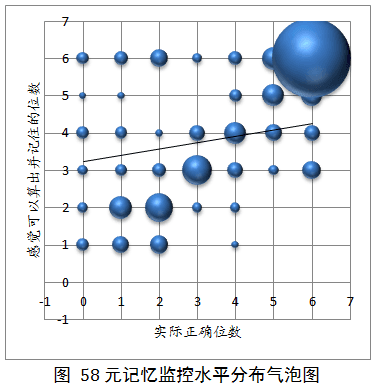
\includegraphics[scale=0.4]{metamemorybubble.png} 
          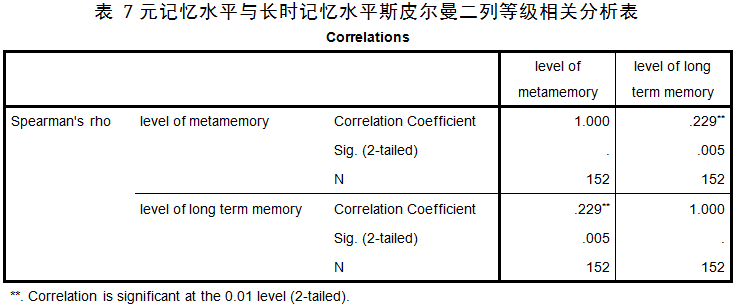
\includegraphics[scale=0.43]{metamemory.png}
          \begin{block}{元记忆相关调查结果}
          	\begin{itemize}
          		\item  \footnotesize {在元记忆对记忆监控低水平的人群中,大部分倾向于乐观高估}
          		\item  \footnotesize {元记忆水平显著影响数学长时记忆的持效性}
          	\end{itemize}
          \end{block} 
    \end{frame}
    
    \begin{frame}{长时工作记忆}
        \begin{columns}
        	\column{0.65\textwidth}
        	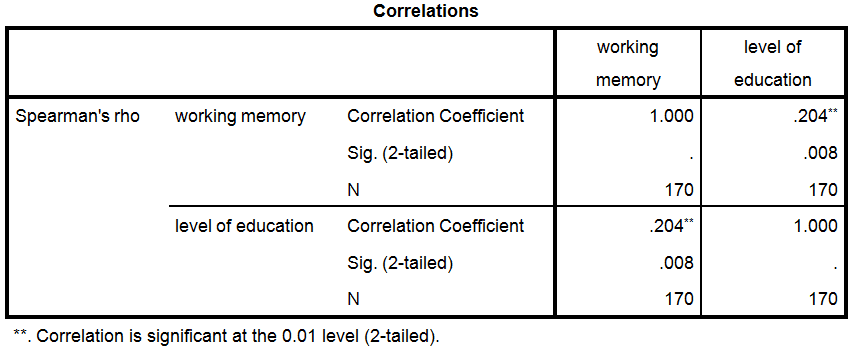
\includegraphics[scale=0.35]{levelofeducation.png} \\
        	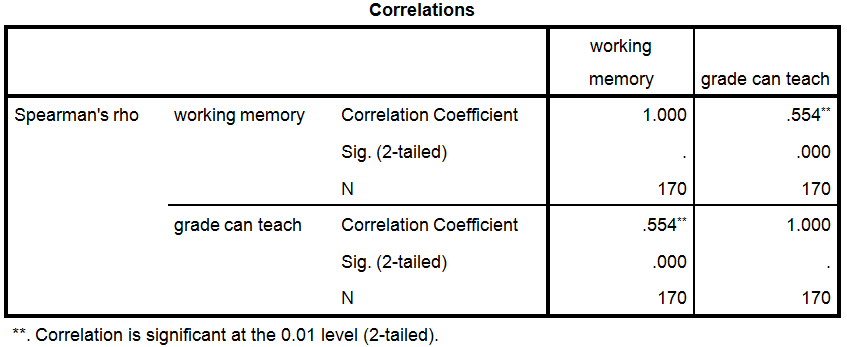
\includegraphics[scale=0.35]{gradecanteach.png}
        	\column{0.35\textwidth}
        	\begin{block}{\small{长时工作记忆相关调查结果}}
        		\begin{itemize}
        			\item  \footnotesize {“专家记忆优势效应”在数学领域同样存在}
        			\item  \footnotesize {高效的提取可以使一部分长时记忆成为工作记忆的有效延伸}
        		\end{itemize}
        	\end{block} 
        \end{columns}
    \end{frame}
    
    \begin{frame}{视觉技能、图象记忆、空间记忆}
        \begin{columns}
    	\column{0.65\textwidth}
    	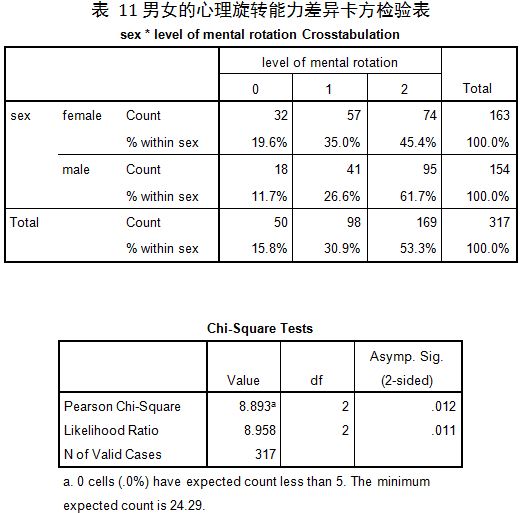
\includegraphics[scale=0.5]{mentalrotation.png}\\
    	\tiny{卡方值为$ 8.893 $,自由度$ df=2 $,$ P=0.012<0.05 $,故有显著性差异 }
    	\column{0.35\textwidth}
    	\begin{block}{\small{心理旋转能力相关调查结果}}
    		\begin{itemize}
    			\item  \footnotesize {男女的心理旋转能力有显著性差异}
    			\item  \footnotesize {能力结构差异使得记忆策略的使用效果因人而异,对记忆策略也有不同偏好}
    		\end{itemize}
    	\end{block} 
        \end{columns}
    \end{frame}
    
    \begin{frame}{视觉技能、图象记忆、空间记忆}
    \begin{columns}
    	\column{0.35\textwidth}
    	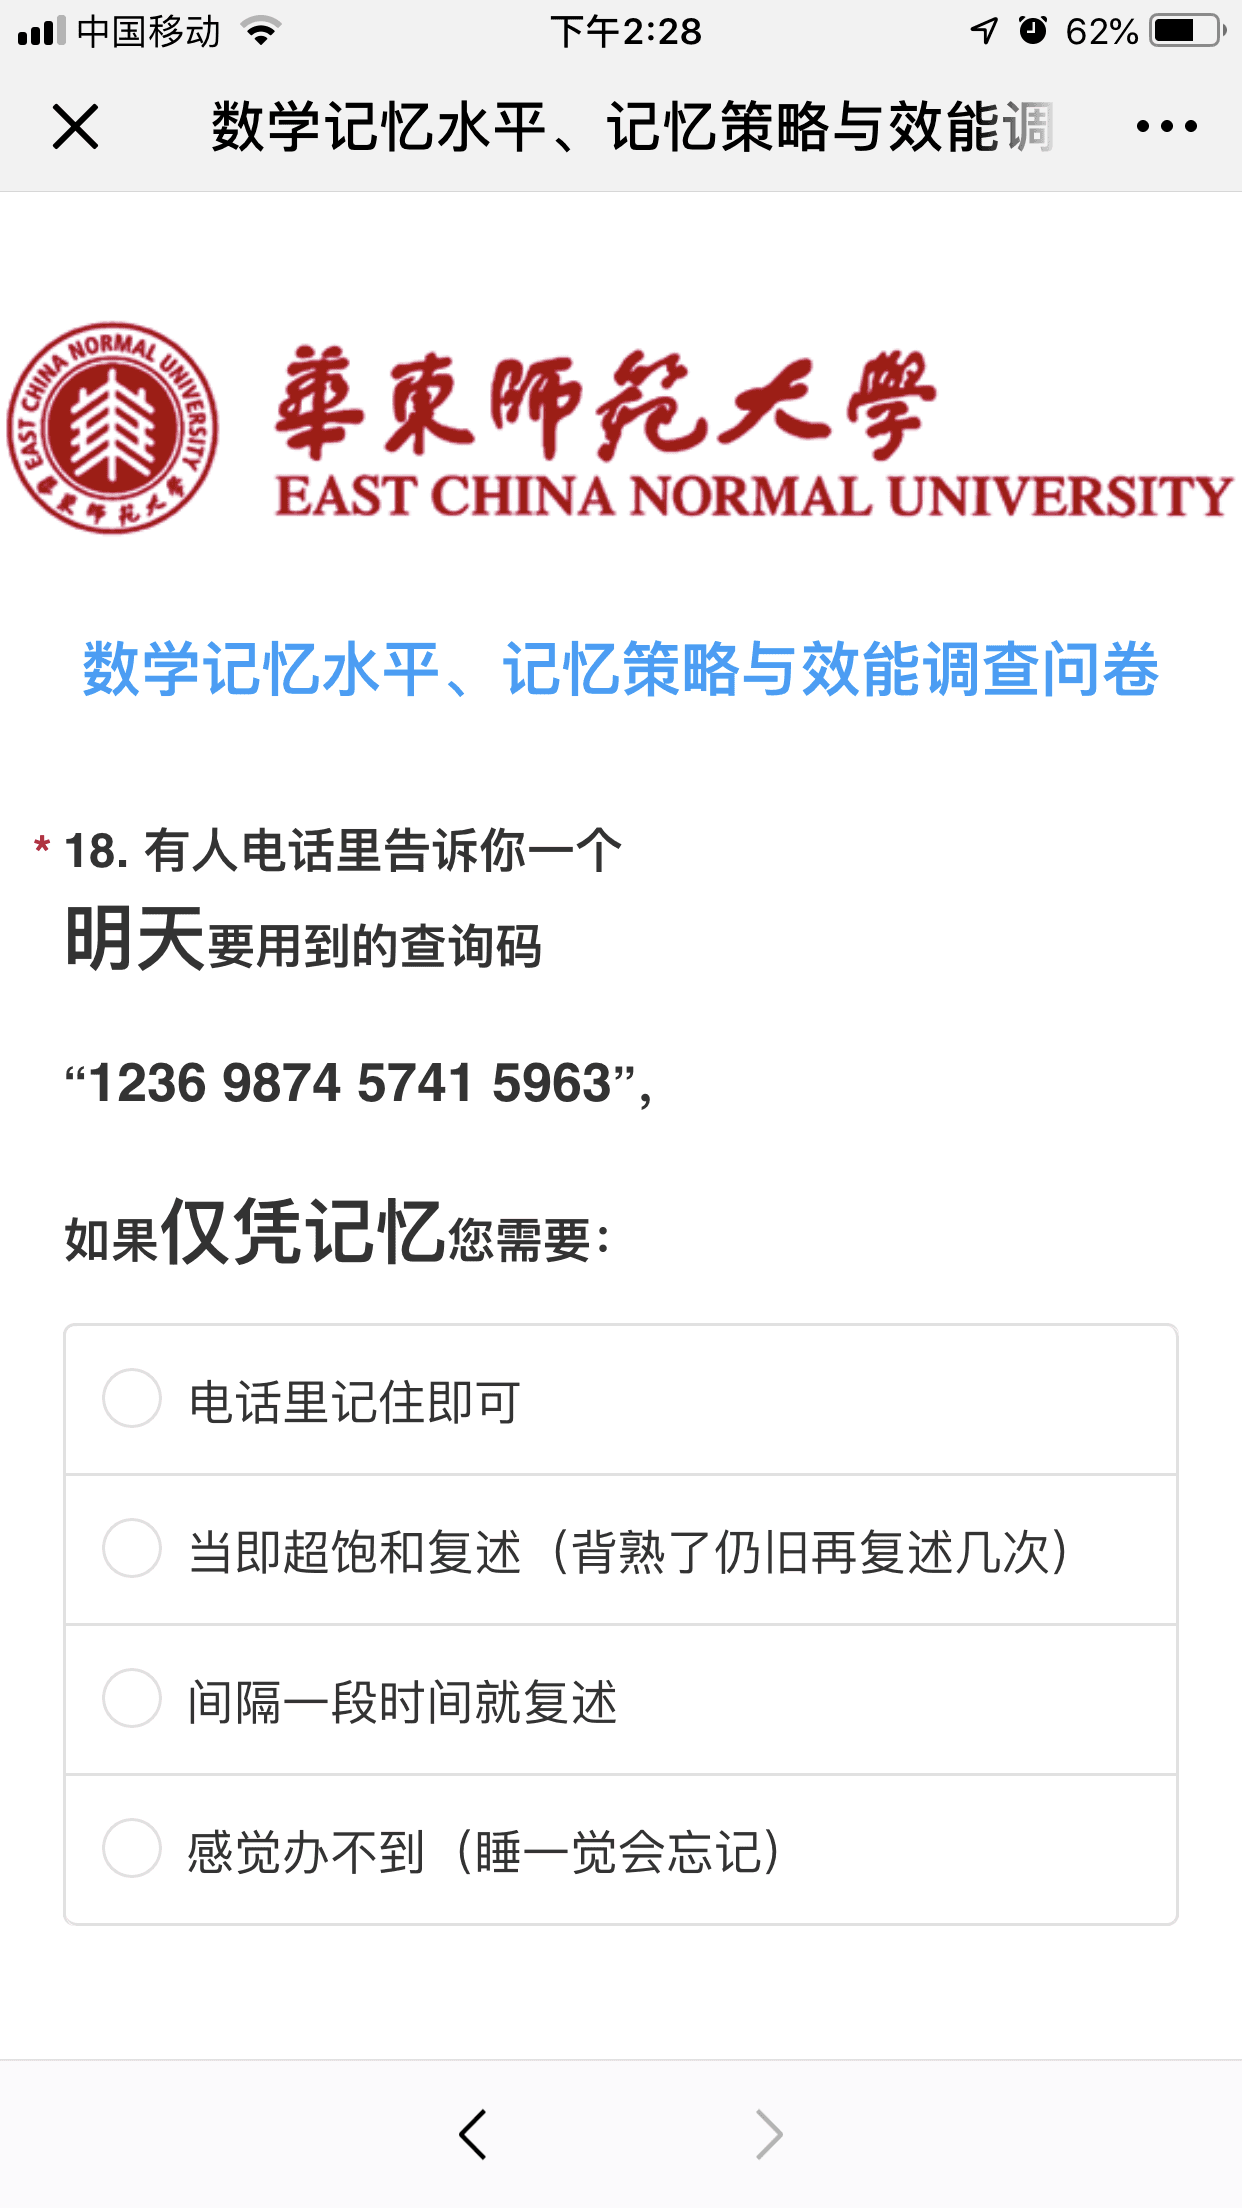
\includegraphics[scale=0.08]{test18.png}\\
    	\scriptsize{仅有13人(约占总人数的4.1\%)}\\
    	\scriptsize{选择第一选项(认为可以比较轻松的记住)}
    	\column{0.35\textwidth}
    	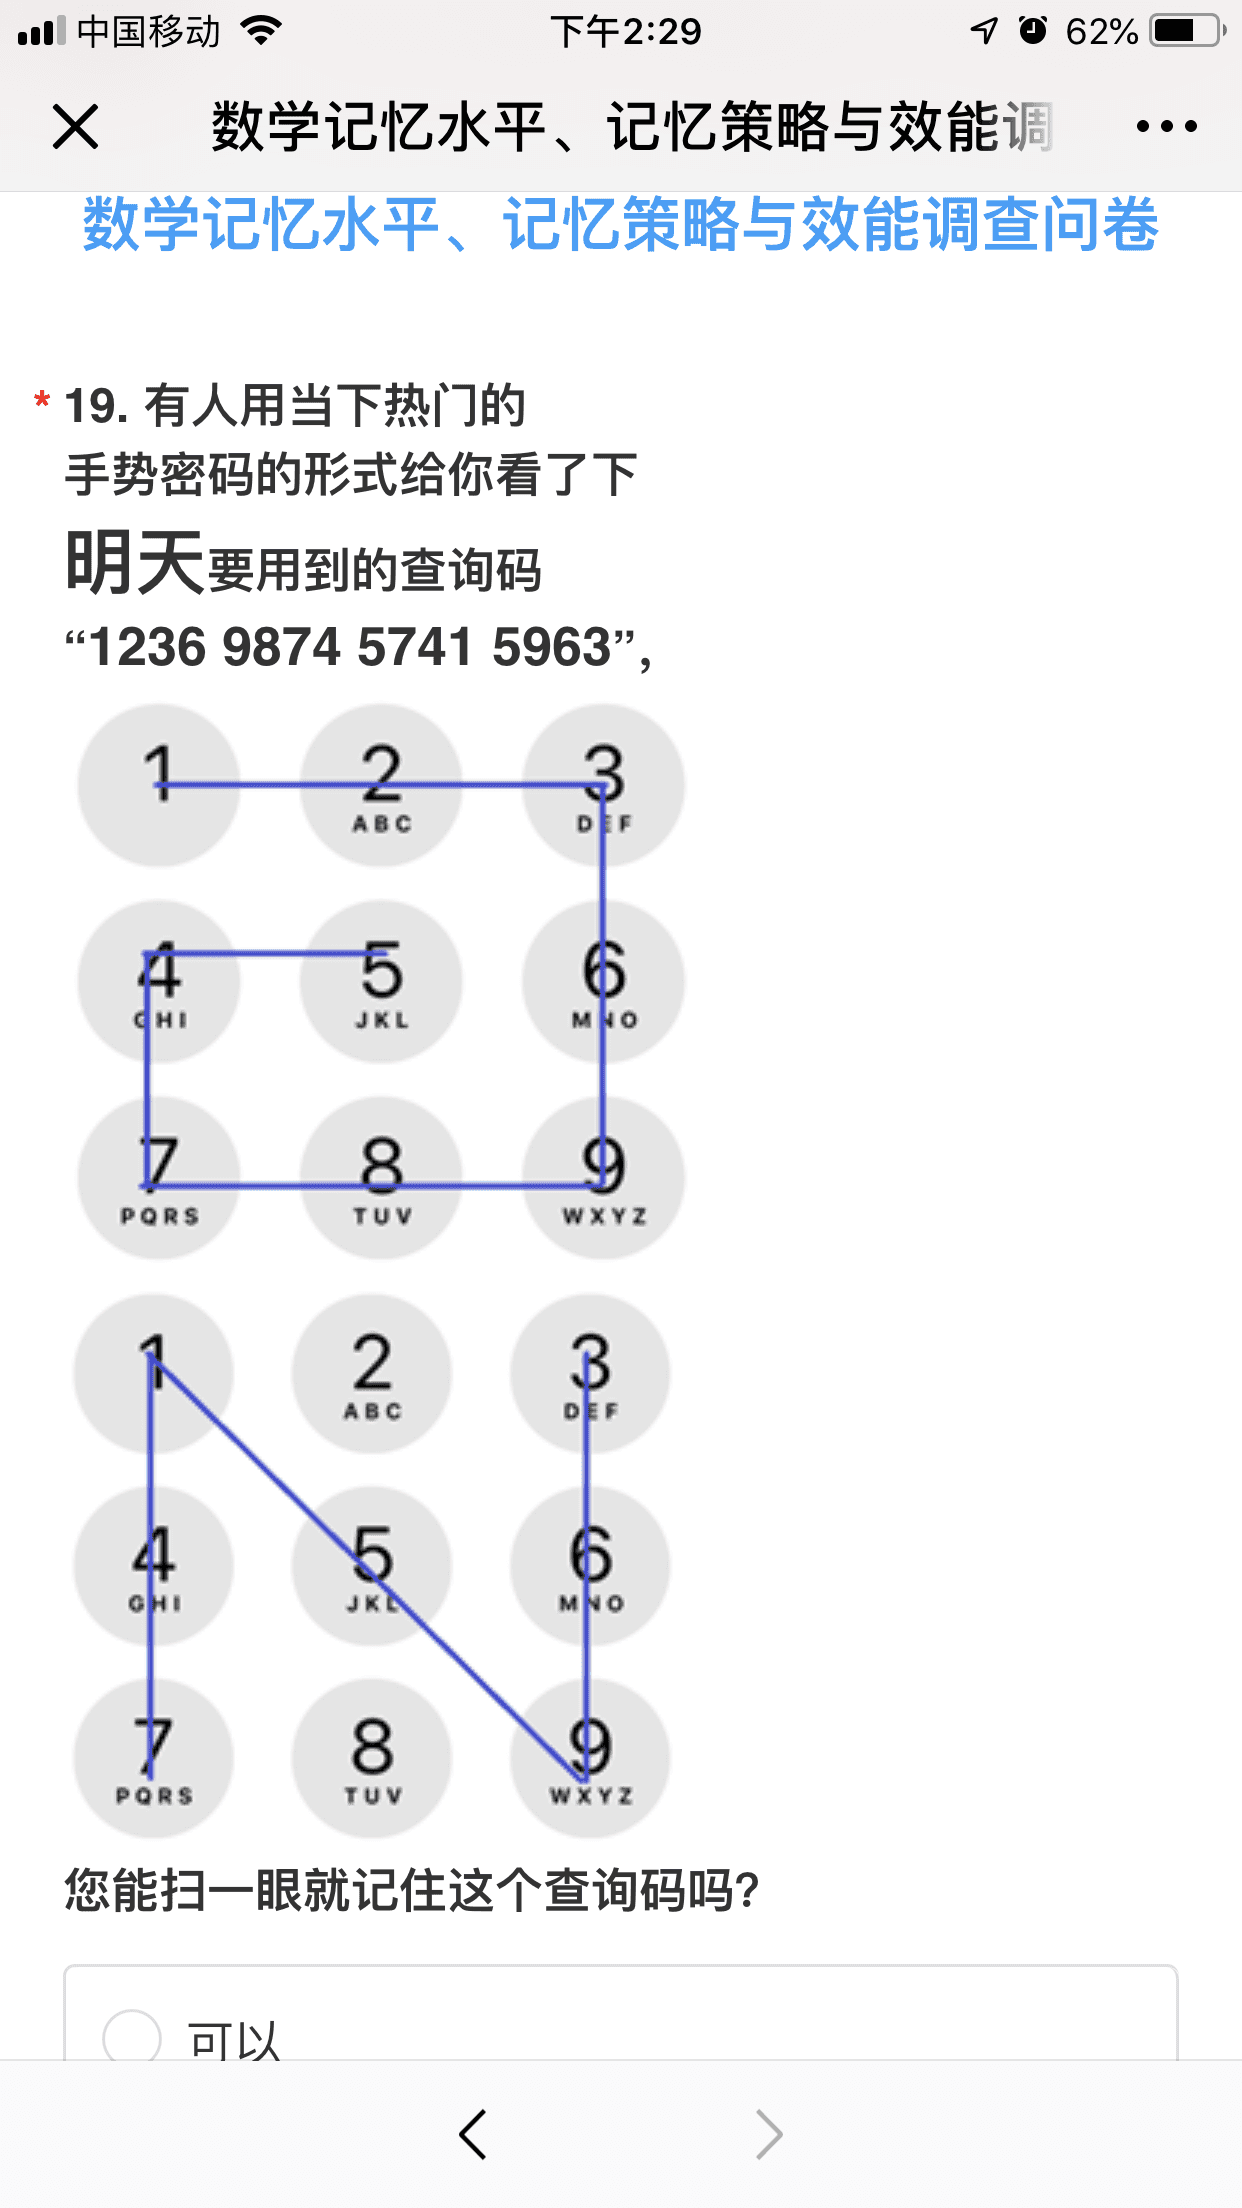
\includegraphics[scale=0.08]{test19.png}\\
    	\scriptsize {有302位(约占总人数的95.3\%)}\\
    	\scriptsize {选择第一选项(认为可以比较轻松的记住)}
    	\column{0.3\textwidth}
    	\begin{block}{结论}
    		合适的记忆策略可以大幅提高记忆效能,视觉技能在记忆中发挥着重要的作用.
    	\end{block}    	
    \end{columns}            
    \end{frame}
    
    \begin{frame}{多重记忆系统}
         \begin{block}{内隐记忆}
        	调查证实记忆确实以多重系统的方式存在,即有需要意识努力的外显记忆,也存在无意间的内隐记忆
         \end{block}
         \pause
         \begin{block}{闪光灯记忆}
    	    调查证实即使关于数学大部分人也存在过闪光灯记忆,这种方式不仅记忆负担轻而且持效性好
         \end{block}
         \pause
         \begin{block}{前瞻记忆}
	        调查证实确有前瞻性记忆水平偏低致使“查漏补缺”、“错题本”也作用不大的情况
         \end{block}
    \end{frame}
    
    \section{课堂教学建议与展望}
    \subsection{课堂教学建议}
    \begin{frame}{建议}
       \begin{enumerate}
       	\item 避免教授碎片化的数学知识
       	\item 注意培养借助符号沟通能力,提高抽象思维能力
       	\item 正视学生个性化差异,呈现多样化记忆策略
       	\item 教学设计兼顾外显记忆与内隐记忆
       	\item 深度加工记忆信息、优化编码、尝试多样化提取
       	\item (热爱运动、科学作息、阳光生活)
       \end{enumerate}
    \end{frame}

    \subsection{展望}
    \begin{frame}{研究中的不足与发展}
        \begin{description}
        	\item[知识结构] 数学教育心理学补短板、科普知识更新、掌握提升效率的教育新技术手段
        	\item[行动研究] 不够深入,将继续“计划--行动--观察--反思--修订计划--行动--观察--反思……”的深入探索,进一步尝试教育实验研究的对比验证
        	\item[调查研究] 变量控制不够严格,样本范围未能做到精准锁定,时限、关联问题设置比较粗放
        \end{description}   
    \end{frame}
    
    \section{致谢}
    \begin{frame}{$ \quad $感谢华东师范大学为我们所创设的系统学习机会}
      \begin{figure}
      	\centering
      	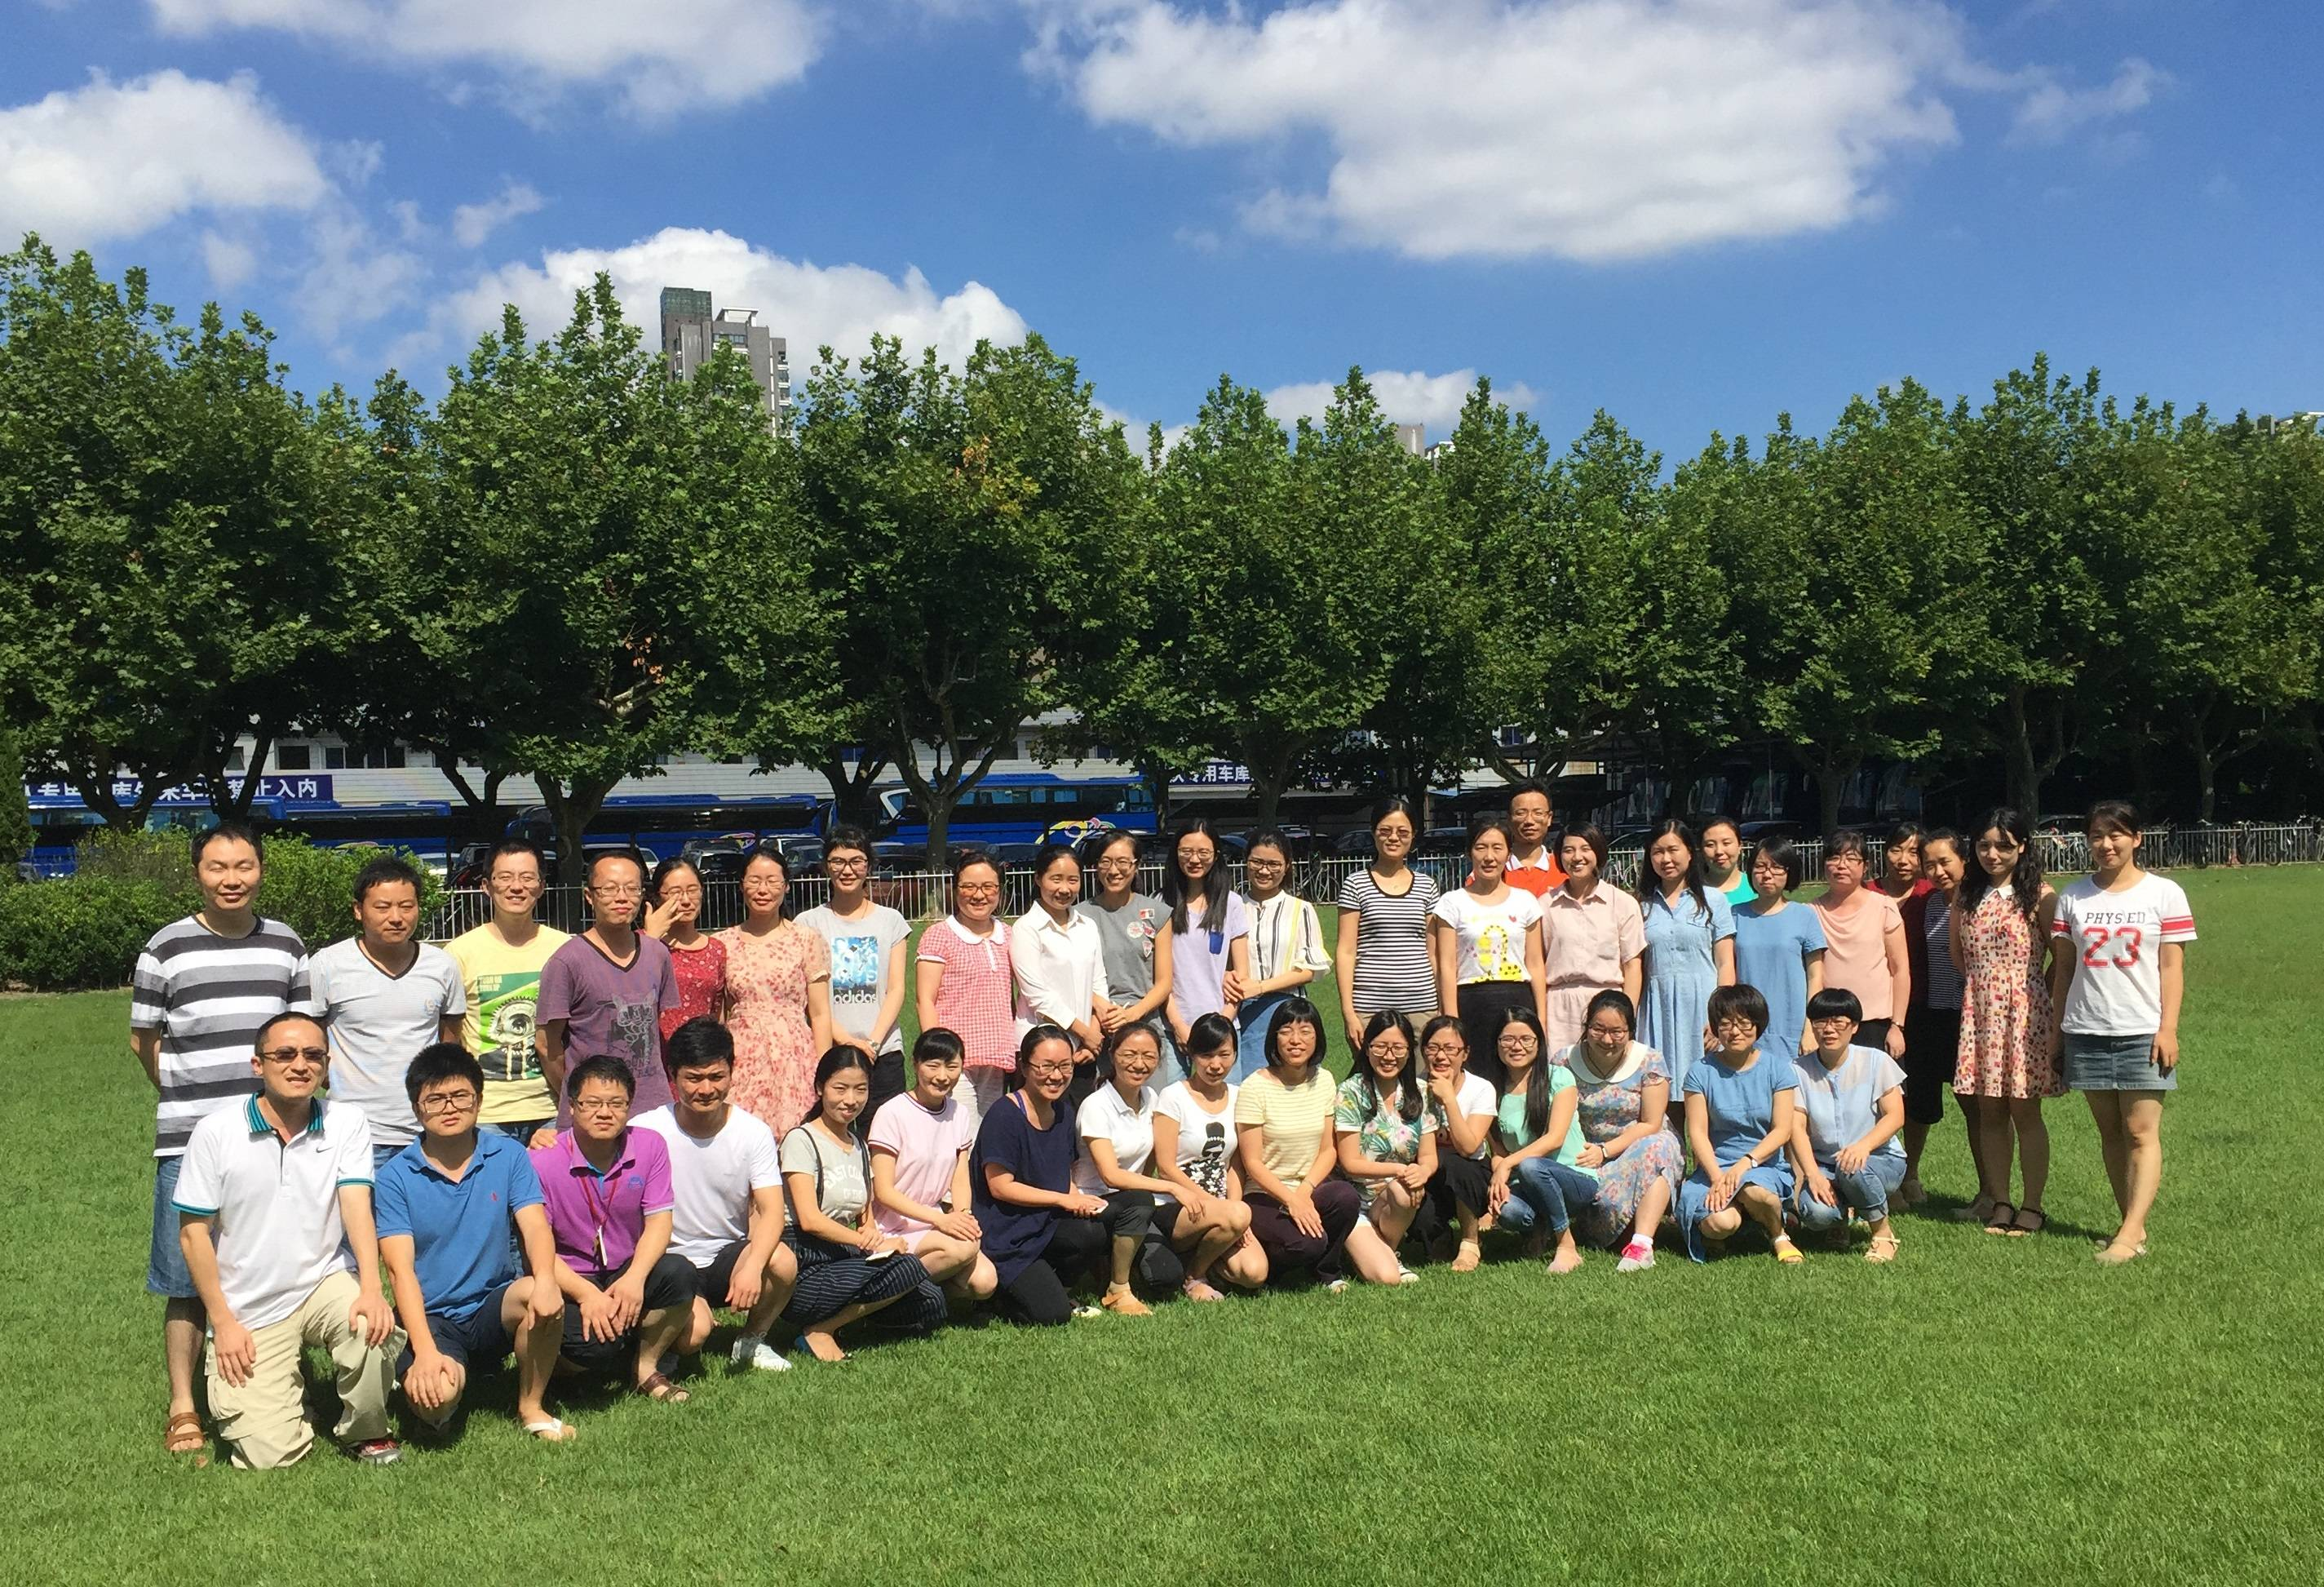
\includegraphics[scale=0.08]{groupphoto.jpg}
      	\caption{\footnotesize{华东师范大学2014、2015级单证在职数学教育硕士(学科教学)合影}}
      \end{figure}   	
    \end{frame}
    
    \begin{frame}{\hspace{\fill}感谢各位专家的指导!}
       \begin{block}{指导老师}
    	熊斌
       \end{block}
       \pause
       \begin{block}{答辩人}
    	徐希来$ \qquad $61150601009$ \qquad $ 学科教学(数学)$ \qquad $ 2015级在职单证
       \end{block}
       \pause
       \begin{figure}[b]
    	\centering
    	
\includegraphics[width=0.32\textwidth]{ECNUred01.jpg}
       \end{figure}
    \end{frame}

\end{document}